\documentclass[11pt,fleqn, openany]{book} % Default font size and left-justified equations

%%%%%%%%%%%%%%%%%%%%%%%%%%%%%%%%%%%%%%%%%
% The Legrand Orange Book
% Structural Definitions File
% Version 2.1 (26/09/2018)
%
% Original author:
% Mathias Legrand (legrand.mathias@gmail.com) with modifications by:
% Vel (vel@latextemplates.com)
% 
% This file was downloaded from:
% http://www.LaTeXTemplates.com
%
% License:
% CC BY-NC-SA 3.0 (http://creativecommons.org/licenses/by-nc-sa/3.0/)
%
%%%%%%%%%%%%%%%%%%%%%%%%%%%%%%%%%%%%%%%%%

%----------------------------------------------------------------------------------------
%	VARIOUS REQUIRED PACKAGES AND CONFIGURATIONS
%----------------------------------------------------------------------------------------

\usepackage[table]{xcolor}

\usepackage{graphicx}
\usepackage{tabularx} % Required for including pictures
\usepackage{pgf,tikz,tkz-tab,eurosym,yhmath, stmaryrd}
\usepackage{pgfplots}
\usepackage{mathrsfs}
\usetikzlibrary{patterns}
\usetikzlibrary{trees}
\graphicspath{{../../Pictures/}}
\usepackage{multicol} 


\usepackage[english]{babel} % English language/hyphenation
\usepackage{icomma}
\usepackage{enumitem} % Customize lists
\setlist{nolistsep, nosep, nolistsep} % Reduce spacing between bullet points and numbered lists

\usepackage{booktabs} % Required for nicer horizontal rules in tables

 % Required for specifying colors by name


\definecolor{ocre}{RGB}{243,102,25} % Define the orange color used for highlighting throughout the book

\usepackage{listings}

\definecolor{codegreen}{rgb}{0,0.6,0}
\definecolor{codegray}{rgb}{0.5,0.5,0.5}
\definecolor{codepurple}{rgb}{0.58,0,0.82}
\definecolor{backcolour}{rgb}{0.95,0.95,0.92}

\lstdefinestyle{mystyle}{
    backgroundcolor=\color{backcolour},   
    commentstyle=\color{codegreen},
    keywordstyle=\color{magenta},
    numberstyle=\tiny\color{codegray},
    stringstyle=\color{codepurple},
    basicstyle=\ttfamily\footnotesize,
    breakatwhitespace=false,         
    breaklines=true,                 
    captionpos=b,                    
    keepspaces=true,                 
    numbers=left,                    
    numbersep=5pt,                  
    showspaces=false,                
    showstringspaces=false,
    showtabs=false,                  
    tabsize=2
}

\lstset{style=mystyle}

%----------------------------------------------------------------------------------------
% Paramétrage XSIM
%----------------------------------------------------------------------------------------

\usepackage[no-files]{xsim}


\DeclareExerciseEnvironmentTemplate{myex}{%
    \textbf{%
      \hypertarget{ex:\ExerciseID}{\sffamily{\ensuremath{\blacktriangleright}} Exercice \GetExerciseProperty{counter} \GetExerciseProperty{subtitle} --}
      \hyperlink{sol:\ExerciseID}{Voir le corrigé}%
    }\par
}{\par\smallskip}

\DeclareExerciseEnvironmentTemplate{mysol}{%
    \textbf{%
      \hypertarget{sol:\ExerciseID}{\sffamily{\ensuremath{\blacktriangleright}} Correction \GetExerciseProperty{counter} --}
      \hyperlink{ex:\ExerciseID}{Voir l'énoncé}%
    }\par
}{\par\medskip}

\xsimsetup{
  exercise/template = myex ,
  solution/template = mysol 
}

%Collection exercices

\DeclareExerciseTagging{topic}

\xsimsetup{collect}

%----------------------------------------------------------------------------------------
% SYMBOLES
%----------------------------------------------------------------------------------------

\newcommand\imCMsym[4][\mathord]{%
  \DeclareFontFamily{U} {#2}{}
  \DeclareFontShape{U}{#2}{m}{n}{
    <-6> #25
    <6-7> #26
    <7-8> #27
    <8-9> #28
    <9-10> #29
    <10-12> #210
    <12-> #212}{}
  \DeclareSymbolFont{CM#2} {U} {#2}{m}{n}
  \DeclareMathSymbol{#4}{#1}{CM#2}{#3}
}
\newcommand\alsoimCMsym[4][\mathord]{\DeclareMathSymbol{#4}{#1}{CM#2}{#3}}

\imCMsym{cmmi}{124}{\CMjmath}

\newcommand{\Oij}{(O\,;\,\vec{\imath}\,,\, \vec{\CMjmath} )}
\newcommand{\Oijk}{(O\,;\,\vec{\imath}\,,\, \vec{\CMjmath}\,,\,\vec{k})}

\newcommand\e{\mathrm{e}}
\newcommand\R{\mathbb{R}}
\newcommand\N{\mathbb{N}}


%----------------------------------------------------------------------------------------
%	MARGINS
%----------------------------------------------------------------------------------------

\usepackage{geometry} % Required for adjusting page dimensions and margins

\geometry{
	paper=a4paper, % Paper size, change to letterpaper for US letter size
	top=3cm, % Top margin
	bottom=3cm, % Bottom margin
	left=2cm, % Left margin
	right=2cm, % Right margin
	headheight=14pt, % Header height
	footskip=1.4cm, % Space from the bottom margin to the baseline of the footer
	headsep=10pt, % Space from the top margin to the baseline of the header
	%showframe, % Uncomment to show how the type block is set on the page
}

\setlength{\parindent}{0pt}
\parskip=5pt



%----------------------------------------------------------------------------------------
%	FONTS
%----------------------------------------------------------------------------------------

\usepackage{avant} % Use the Avantgarde font for headings
\usepackage{times} % Use the Times font for headings
\usepackage{mathptmx} % Use the Adobe Times Roman as the default text font together with math symbols from the Sym­bol, Chancery and Com­puter Modern fonts

%\usepackage{microtype} % Slightly tweak font spacing for aesthetics
%\usepackage[utf8]{inputenc} % Required for including letters with accents
\usepackage[T1]{fontenc} % Use 8-bit encoding that has 256 glyphs

%----------------------------------------------------------------------------------------
%	BIBLIOGRAPHY AND INDEX
%----------------------------------------------------------------------------------------

\usepackage[style=numeric,citestyle=numeric,sorting=nyt,sortcites=true,autopunct=true,babel=hyphen,hyperref=true,abbreviate=false,backref=true,backend=biber]{biblatex}
\addbibresource{bibliography.bib} % BibTeX bibliography file
\defbibheading{bibempty}{}

\usepackage{calc} % For simpler calculation - used for spacing the index letter headings correctly
\usepackage{makeidx} % Required to make an index
\makeindex % Tells LaTeX to create the files required for indexing

%----------------------------------------------------------------------------------------
%	MAIN TABLE OF CONTENTS
%----------------------------------------------------------------------------------------

\usepackage{titletoc} % Required for manipulating the table of contents

\contentsmargin{0cm} % Removes the default margin

% Part text styling (this is mostly taken care of in the PART HEADINGS section of this file)
\titlecontents{part}
	[0cm] % Left indentation
	{\addvspace{20pt}\bfseries} % Spacing and font options for parts
	{}
	{}
	{}

% Chapter text styling
\titlecontents{chapter}
	[1.25cm] % Left indentation
	{\addvspace{12pt}\large\sffamily\bfseries} % Spacing and font options for chapters
	{\color{ocre!60}\contentslabel[\Large\thecontentslabel]{1.25cm}\color{ocre}} % Formatting of numbered sections of this type
	{\color{ocre}} % Formatting of numberless sections of this type
	{\color{ocre!60}\normalsize\;\titlerule*[.5pc]{.}\;\thecontentspage} % Formatting of the filler to the right of the heading and the page number

% Section text styling
\titlecontents{section}
	[1.25cm] % Left indentation
	{\addvspace{3pt}\sffamily\bfseries} % Spacing and font options for sections
	{\contentslabel[\thecontentslabel]{1.25cm}} % Formatting of numbered sections of this type
	{} % Formatting of numberless sections of this type
	{\hfill\color{black}\thecontentspage} % Formatting of the filler to the right of the heading and the page number

% Subsection text styling
\titlecontents{subsection}
	[1.25cm] % Left indentation
	{\addvspace{1pt}\sffamily\small} % Spacing and font options for subsections
	{\contentslabel[\thecontentslabel]{1.25cm}} % Formatting of numbered sections of this type
	{} % Formatting of numberless sections of this type
	{\ \titlerule*[.5pc]{.}\;\thecontentspage} % Formatting of the filler to the right of the heading and the page number

% Figure text styling
\titlecontents{figure}
	[1.25cm] % Left indentation
	{\addvspace{1pt}\sffamily\small} % Spacing and font options for figures
	{\thecontentslabel\hspace*{1em}} % Formatting of numbered sections of this type
	{} % Formatting of numberless sections of this type
	{\ \titlerule*[.5pc]{.}\;\thecontentspage} % Formatting of the filler to the right of the heading and the page number

% Table text styling
\titlecontents{table}
	[1.25cm] % Left indentation
	{\addvspace{1pt}\sffamily\small} % Spacing and font options for tables
	{\thecontentslabel\hspace*{1em}} % Formatting of numbered sections of this type
	{} % Formatting of numberless sections of this type
	{\ \titlerule*[.5pc]{.}\;\thecontentspage} % Formatting of the filler to the right of the heading and the page number

%----------------------------------------------------------------------------------------
%	MINI TABLE OF CONTENTS IN PART HEADS
%----------------------------------------------------------------------------------------

% Chapter text styling
\titlecontents{lchapter}
	[0em] % Left indentation
	{\addvspace{15pt}\large\sffamily\bfseries} % Spacing and font options for chapters
	{\color{ocre}\contentslabel[\Large\thecontentslabel]{1.25cm}\color{ocre}} % Chapter number
	{}  
	{\color{ocre}\normalsize\sffamily\bfseries\;\titlerule*[.5pc]{.}\;\thecontentspage} % Page number

% Section text styling
\titlecontents{lsection}
	[0em] % Left indentation
	{\sffamily\small} % Spacing and font options for sections
	{\contentslabel[\thecontentslabel]{1.25cm}} % Section number
	{}
	{}

% Subsection text styling (note these aren't shown by default, display them by searchings this file for tocdepth and reading the commented text)
\titlecontents{lsubsection}
	[.5em] % Left indentation
	{\sffamily\footnotesize} % Spacing and font options for subsections
	{\contentslabel[\thecontentslabel]{1.25cm}}
	{}
	{}

%----------------------------------------------------------------------------------------
%	HEADERS AND FOOTERS
%----------------------------------------------------------------------------------------


\usepackage{fancyhdr} % Required for header and footer configuration

\pagestyle{fancy}
\renewcommand{\chaptermark}[1]{\markboth{\sffamily\normalsize\bfseries\ \thechapter.\ #1}{}} % Chapter text font settings
\renewcommand{\sectionmark}[1]{\markright{\sffamily\normalsize\thesection\hspace{5pt}#1}{}} % Section text font settings
\fancyhf{} \fancyhead[LE,RO]{\sffamily\normalsize\thepage} % Font setting for the page number in the header
\fancyhead[LO]{\rightmark} % Print the nearest section name on the left side of odd pages
\fancyhead[RE]{\leftmark} % Print the current chapter name on the right side of even pages

\fancyfoot[L]{Jason LAPEYRONNIE}
\fancyfoot[R]{\href{http://mathoutils.fr}{http://mathoutils.fr}} % Uncomment to include a footer

\renewcommand{\headrulewidth}{0.5pt} % Thickness of the rule under the header
\renewcommand{\footrulewidth}{0.5pt} % Thickness of the rule under the header

\fancypagestyle{plain}{% Style for when a plain pagestyle is specified
	\fancyhead{}\renewcommand{\headrulewidth}{0pt}%
}

% Removes the header from odd empty pages at the end of chapters
\makeatletter
\renewcommand{\cleardoublepage}{
\clearpage\ifodd\c@page\else
\hbox{}
\vspace*{\fill}
\thispagestyle{empty}
\newpage
\fi}

%----------------------------------------------------------------------------------------
%	THEOREM STYLES
%----------------------------------------------------------------------------------------

\usepackage{amsmath,amsfonts,amssymb,amsthm} % For math equations, theorems, symbols, etc

\newcommand{\intoo}[2]{\mathopen{]}#1\,;#2\mathclose{[}}
\newcommand{\ud}{\mathop{\mathrm{{}d}}\mathopen{}}
\newcommand{\intff}[2]{\mathopen{[}#1\,;#2\mathclose{]}}
\renewcommand{\qedsymbol}{$\blacksquare$}
\newtheorem{notation}{Notation}[section]

% Boxed/framed environments
\newtheoremstyle{ocrenumbox}% Theorem style name
{0pt}% Space above
{0pt}% Space below
{\normalfont}% Body font
{}% Indent amount
{\small\bf\sffamily\color{ocre}}% Theorem head font
{\;:\;}% Punctuation after theorem head
{0.25em}% Space after theorem head
{\small\sffamily\color{ocre}\thmname{#1}\nobreakspace\thmnumber{\@ifnotempty{#1}{}\@upn{#2}}% Theorem text (e.g. Theorem 2.1)
\thmnote{\nobreakspace\the\thm@notefont\sffamily\bfseries\color{black}---\nobreakspace#3}} % Optional theorem note

\newtheoremstyle{blacknumex}% Theorem style name
{5pt}% Space above
{10pt}% Space below
{\normalfont}% Body font
{} % Indent amount
{\small\bf\sffamily}% Theorem head font
{\;:\;}% Punctuation after theorem head
{0.25em}% Space after theorem head
{\small\sffamily{\tiny\ensuremath{\blacksquare}}\nobreakspace\thmname{#1}\nobreakspace\thmnumber{\@ifnotempty{#1}{}\@upn{#2}}% Theorem text (e.g. Theorem 2.1)
\thmnote{\nobreakspace\the\thm@notefont\sffamily\bfseries---\nobreakspace#3}}% Optional theorem note

\newtheoremstyle{blacknumexo}% Theorem style name
{15pt}% Space above
{10pt}% Space below
{\normalfont}% Body font
{} % Indent amount
{\small\bf\sffamily}% Theorem head font
{}% Punctuation after theorem head
{0.5em}% Space after theorem head
{\small\sffamily{\ensuremath{\blacktriangleright}}\nobreakspace\thmname{#1}\nobreakspace\thmnumber{\@ifnotempty{#1}{}\@upn{#2}}% Theorem text (e.g. Theorem 2.1)
\thmnote{\nobreakspace\the\thm@notefont\sffamily\bfseries---\nobreakspace#3} \\}% Optional theorem note



\newtheoremstyle{blacknumbox} % Theorem style name
{0pt}% Space above
{5pt}% Space below
{}% Body font
{}% Indent amount
{\large\bf\sffamily}% Theorem head font
{\;:\;}% Punctuation after theorem head
{0.25em}% Space after theorem head
{\small\sffamily\thmname{#1}\nobreakspace\thmnumber{\@ifnotempty{#1}{}\@upn{#2}}% Theorem text (e.g. Theorem 2.1)
\thmnote{\nobreakspace\the\thm@notefont\sffamily\bfseries---\nobreakspace#3}}% Optional theorem note

% Non-boxed/non-framed environments
\newtheoremstyle{ocrenum}% Theorem style name
{5pt}% Space above
{5pt}% Space below
{\normalfont}% Body font
{}% Indent amount
{\small\bf\sffamily\color{ocre}}% Theorem head font
{\;:\;}% Punctuation after theorem head
{0.25em}% Space after theorem head
{\small\sffamily\color{ocre}\thmname{#1}\nobreakspace\thmnumber{\@ifnotempty{#1}{}\@upn{#2}}% Theorem text (e.g. Theorem 2.1)
\thmnote{\nobreakspace\the\thm@notefont\sffamily\bfseries\color{black}---\nobreakspace#3}} % Optional theorem note
\makeatother

% Defines the theorem text style for each type of theorem to one of the three styles above
\newcounter{dummy} 
\newcounter{thm}
\newcounter{correction}
\newcounter{qst}
\theoremstyle{ocrenumbox}
\newtheorem{theoremeT}[dummy]{Théorème}
\newtheorem{exerciseT}{Propriété}
\newtheorem{principeT}{Principe}
\theoremstyle{blacknumex}
\newtheorem{exampleT}{Exemple}
\theoremstyle{blacknumexo}
\newtheorem{exo}[thm]{Exercice}
\newtheorem{corr}[correction]{Correction}
\newtheorem{quest}[qst]{Question}
\theoremstyle{blacknumbox}
\newtheorem{vocabulary}{Vocabulary}[section]
\newtheorem{definitionT}{Définition}
\newtheorem{corollaryT}[dummy]{Corollary}
\theoremstyle{ocrenum}
\newtheorem{proofT}[dummy]{Démonstration}


%----------------------------------------------------------------------------------------
%	DEFINITION OF COLORED BOXES
%----------------------------------------------------------------------------------------

\RequirePackage[framemethod=default]{mdframed} % Required for creating the theorem, definition, exercise and corollary boxes

% Theorem box
\newmdenv[skipabove=7pt,
skipbelow=7pt,
backgroundcolor=black!5,
linecolor=ocre,
innerleftmargin=5pt,
innerrightmargin=5pt,
innertopmargin=10pt,
leftmargin=0cm,
rightmargin=0cm,
innerbottommargin=5pt]{tBox}

%Proposition box	  
\newmdenv[skipabove=7pt,
skipbelow=7pt,
rightline=false,
leftline=true,
topline=false,
bottomline=false,
backgroundcolor=ocre!10,
linecolor=ocre,
innerleftmargin=5pt,
innerrightmargin=5pt,
innertopmargin=10pt,
innerbottommargin=3pt,
leftmargin=0cm,
rightmargin=0cm,
linewidth=4pt]{eBox}	

% Definition box
\newmdenv[skipabove=7pt,
backgroundcolor=ocre!4,
skipbelow=7pt,
rightline=false,
leftline=true,
topline=false,
bottomline=false,
linecolor=ocre,
innerleftmargin=5pt,
innerrightmargin=5pt,
innertopmargin=10pt,
leftmargin=0cm,
rightmargin=0cm,
linewidth=4pt,
innerbottommargin=5pt]{dBox}	

% Corollary box
\newmdenv[skipabove=7pt,
skipbelow=7pt,
rightline=false,
leftline=true,
topline=false,
bottomline=false,
linecolor=gray,
backgroundcolor=black!5,
innerleftmargin=5pt,
innerrightmargin=5pt,
innertopmargin=5pt,
leftmargin=0cm,
rightmargin=0cm,
linewidth=4pt,
innerbottommargin=5pt]{cBox}

\newmdenv[skipabove=7pt,
skipbelow=7pt,
backgroundcolor=black!5,
innerleftmargin=5pt,
topline=false,
bottomline=false,
rightline=false,
leftline=false,
innerrightmargin=5pt,
innertopmargin=5pt,
leftmargin=0cm,
rightmargin=0cm,
innerbottommargin=5pt]{xBox}

% Creates an environment for each type of theorem and assigns it a theorem text style from the "Theorem Styles" section above and a colored box from above
\newenvironment{theorem}{\begin{tBox}\begin{theoremeT}}{\end{theoremeT}\end{tBox}}

\newenvironment{exo2}{\noindent \begin{exo}\item\relax \noindent \begin{eBox}\item\relax}{\end{eBox}\end{exo}}


\newenvironment{proposition}{\begin{eBox}\begin{exerciseT}}{\hfill{\color{ocre}}\end{exerciseT}\end{eBox}}		

\newenvironment{principe}{\begin{eBox}\begin{principeT}}{\hfill{\color{ocre}}\end{principeT}\end{eBox}}	
		  
\newenvironment{definition}{\begin{dBox}\begin{definitionT}}{\end{definitionT}\end{dBox}}	

\newenvironment{example}{\begin{xBox}\begin{exampleT}}{\hfill{\tiny\ensuremath{\blacksquare}}\end{exampleT}\end{xBox}}

\newenvironment{demonstration}{\begin{proofT}}{\hfill{\tiny\ensuremath{\square}}\end{proofT}}		
\newenvironment{corollary}{\begin{cBox}\begin{corollaryT}}{\end{corollaryT}\end{cBox}}	

%----------------------------------------------------------------------------------------
%	REMARK ENVIRONMENT
%----------------------------------------------------------------------------------------

\newenvironment{remark}{\par\vspace{5pt}\small % Vertical white space above the remark and smaller font size
\begin{list}{}{
\leftmargin=25pt % Indentation on the left
\rightmargin=15pt}\item\ignorespaces % Indentation on the right
\makebox[-2.5pt]{
\begin{tikzpicture}[overlay]
\node[draw=ocre!60,line width=1pt,circle,fill=ocre!25,font=\sffamily\bfseries,inner sep=2pt,outer sep=0pt] at (-15pt,0pt){\textcolor{ocre}{R}};\end{tikzpicture}} % Orange R in a circle
\advance\baselineskip -1pt}{\end{list}\vskip5pt} % Tighter line spacing and white space after remark

%----------------------------------------------------------------------------------------
%	SECTION NUMBERING IN THE MARGIN
%----------------------------------------------------------------------------------------

\makeatletter
\renewcommand{\@seccntformat}[1]{\llap{\textcolor{ocre}{\csname the#1\endcsname}\hspace{1em}}}                    
\renewcommand{\section}{\@startsection{section}{1}{\z@}
{-4ex \@plus -1ex \@minus -.4ex}
{1ex \@plus.2ex }
{\normalfont\LARGE\sffamily\bfseries}}
\renewcommand{\subsection}{\@startsection {subsection}{2}{\z@}
{-3ex \@plus -0.1ex \@minus -.4ex}
{0.5ex \@plus.2ex }
{\normalfont\sffamily\bfseries}}
\renewcommand{\subsubsection}{\@startsection {subsubsection}{3}{\z@}
{-2ex \@plus -0.1ex \@minus -.2ex}
{.2ex \@plus.2ex }
{\normalfont\small\sffamily\bfseries}}                        
\renewcommand\paragraph{\@startsection{paragraph}{4}{\z@}
{-2ex \@plus-.2ex \@minus .2ex}
{.1ex}
{\normalfont\small\sffamily\bfseries}}

%----------------------------------------------------------------------------------------
%	PART HEADINGS
%----------------------------------------------------------------------------------------

% Numbered part in the table of contents
\newcommand{\@mypartnumtocformat}[2]{%
	\setlength\fboxsep{0pt}%
	\noindent\colorbox{ocre!20}{\strut\parbox[c][.7cm]{\ecart}{\color{ocre!70}\Large\sffamily\bfseries\centering#1}}\hskip\esp\colorbox{ocre!40}{\strut\parbox[c][.7cm]{\linewidth-\ecart-\esp}{\Large\sffamily\centering#2}}%
}

% Unnumbered part in the table of contents
\newcommand{\@myparttocformat}[1]{%
	\setlength\fboxsep{0pt}%
	\noindent\colorbox{ocre!40}{\strut\parbox[c][.7cm]{\linewidth}{\Large\sffamily\centering#1}}%
}

\newlength\esp
\setlength\esp{4pt}
\newlength\ecart
\setlength\ecart{1.2cm-\esp}
\newcommand{\thepartimage}{}%
\newcommand{\partimage}[1]{\renewcommand{\thepartimage}{#1}}%
\def\@part[#1]#2{%
\ifnum \c@secnumdepth >-2\relax%
\refstepcounter{part}%
\addcontentsline{toc}{part}{\texorpdfstring{\protect\@mypartnumtocformat{\thepart}{#1}}{\partname~\thepart\ ---\ #1}}
\else%
\addcontentsline{toc}{part}{\texorpdfstring{\protect\@myparttocformat{#1}}{#1}}%
\fi%
\startcontents%
\markboth{}{}%
{\thispagestyle{empty}%
\begin{tikzpicture}[remember picture,overlay]%
\node at (current page.north west){\begin{tikzpicture}[remember picture,overlay]%	
\fill[ocre!20](0cm,0cm) rectangle (\paperwidth,-\paperheight);
\node[anchor=north] at (4cm,-3.25cm){\color{ocre!40}\fontsize{220}{100}\sffamily\bfseries\thepart}; 
\node[anchor=south east] at (\paperwidth-1cm,-\paperheight+1cm){\parbox[t][][t]{8.5cm}{
\printcontents{l}{0}{\setcounter{tocdepth}{1}}% The depth to which the Part mini table of contents displays headings; 0 for chapters only, 1 for chapters and sections and 2 for chapters, sections and subsections
}};
\node[anchor=north east] at (\paperwidth-1.5cm,-3.25cm){\parbox[t][][t]{15cm}{\strut\raggedleft\color{white}\fontsize{30}{30}\sffamily\bfseries#2}};
\end{tikzpicture}};
\end{tikzpicture}}%
\@endpart}
\def\@spart#1{%
\startcontents%
\phantomsection
{\thispagestyle{empty}%
\begin{tikzpicture}[remember picture,overlay]%
\node at (current page.north west){\begin{tikzpicture}[remember picture,overlay]%	
\fill[ocre!20](0cm,0cm) rectangle (\paperwidth,-\paperheight);
\node[anchor=north east] at (\paperwidth-1.5cm,-3.25cm){\parbox[t][][t]{15cm}{\strut\raggedleft\color{white}\fontsize{30}{30}\sffamily\bfseries#1}};
\end{tikzpicture}};
\end{tikzpicture}}
\addcontentsline{toc}{part}{\texorpdfstring{%
\setlength\fboxsep{0pt}%
\noindent\protect\colorbox{ocre!40}{\strut\protect\parbox[c][.7cm]{\linewidth}{\Large\sffamily\protect\centering #1\quad\mbox{}}}}{#1}}%
\@endpart}
\def\@endpart{\vfil\newpage
\if@twoside
\if@openright
\null
\thispagestyle{empty}%
\newpage
\fi
\fi
\if@tempswa
\twocolumn
\fi}

%----------------------------------------------------------------------------------------
%	CHAPTER HEADINGS
%----------------------------------------------------------------------------------------

% A switch to conditionally include a picture, implemented by Christian Hupfer
\newif\ifusechapterimage
\usechapterimagetrue
\newcommand{\thechapterimage}{}%
\newcommand{\chapterimage}[1]{\ifusechapterimage\renewcommand{\thechapterimage}{#1}\fi}%
\newcommand{\autodot}{.}
\def\@makechapterhead#1{%
{\parindent \z@ \raggedright \normalfont
\ifnum \c@secnumdepth >\m@ne
\if@mainmatter
\begin{tikzpicture}[remember picture,overlay]
\node at (current page.north west)
{\begin{tikzpicture}[remember picture,overlay]
\node[anchor=north west,inner sep=0pt] at (0,0) {\ifusechapterimage\includegraphics[width=\paperwidth]{\thechapterimage}\fi};
\draw[anchor=west] (\Gm@lmargin,-3cm) node [line width=2pt,rounded corners=15pt,draw=ocre,fill=white,fill opacity=0.5,inner sep=15pt]{\strut\makebox[22cm]{}};
\draw[anchor=west] (\Gm@lmargin+.3cm,-3cm) node {\huge\sffamily\bfseries\color{black}\thechapter\autodot~#1\strut};
\end{tikzpicture}};
\end{tikzpicture}
\else
\begin{tikzpicture}[remember picture,overlay]
\node at (current page.north west)
{\begin{tikzpicture}[remember picture,overlay]
\node[anchor=north west,inner sep=0pt] at (0,0) {\ifusechapterimage\includegraphics[width=\paperwidth]{\thechapterimage}\fi};
\draw[anchor=west] (\Gm@lmargin,-3cm) node [line width=2pt,rounded corners=15pt,draw=ocre,fill=white,fill opacity=0.5,inner sep=15pt]{\strut\makebox[22cm]{}};
\draw[anchor=west] (\Gm@lmargin+.3cm,-3cm) node {\huge\sffamily\bfseries\color{black}#1\strut};
\end{tikzpicture}};
\end{tikzpicture}
\fi\fi\par\vspace*{50\p@}}}

%-------------------------------------------

\def\@makeschapterhead#1{%
\begin{tikzpicture}[remember picture,overlay]
\node at (current page.north west)
{\begin{tikzpicture}[remember picture,overlay]
\node[anchor=north west,inner sep=0pt] at (0,0) {\ifusechapterimage\includegraphics[width=\paperwidth]{\thechapterimage}\fi};
\draw[anchor=west] (\Gm@lmargin,-3cm) node [line width=2pt,rounded corners=15pt,draw=ocre,fill=white,fill opacity=0.5,inner sep=15pt]{\strut\makebox[22cm]{}};
\draw[anchor=west] (\Gm@lmargin+.3cm,-3cm) node {\huge\sffamily\bfseries\color{black}#1\strut};
\end{tikzpicture}};
\end{tikzpicture}
\par\vspace*{50\p@}}
\makeatother

%----------------------------------------------------------------------------------------
%	LINKS
%----------------------------------------------------------------------------------------

\usepackage{hyperref}
\hypersetup{hidelinks,backref=true,pagebackref=true,hyperindex=true,colorlinks=false,breaklinks=true,urlcolor=ocre,bookmarks=true,bookmarksopen=false}

\usepackage{bookmark}
\bookmarksetup{
open,
numbered,
addtohook={%
\ifnum\bookmarkget{level}=0 % chapter
\bookmarksetup{bold}%
\fi
\ifnum\bookmarkget{level}=-1 % part
\bookmarksetup{color=ocre,bold}%
\fi
}
}

\renewcommand*\thesection{\arabic{section}}

\newcommand*{\coord}[3]{% 
  \ensuremath{\overrightarrow{#1}\, 
    \begin{pmatrix} 
      #2\\ 
      #3 
    \end{pmatrix}}}
    
  \newcommand*{\coordb}[2]{% 
  \ensuremath{ 
    \begin{pmatrix} 
      #1\\ 
      #2 
    \end{pmatrix}}}

\newcommand*{\coorde}[4]{% 
  \renewcommand{\arraystretch}{1}\ensuremath{\overrightarrow{#1}\, 
    \begin{pmatrix} 
      #2\\ 
      #3 \\
      #4
    \end{pmatrix}}}    
  \newcommand*{\coordbe}[3]{% 
 \renewcommand{\arraystretch}{1} \ensuremath{ 
    \begin{pmatrix} 
      #1\\ 
      #2 \\
      #3
    \end{pmatrix}}}  
    
\newcommand{\Card}{\mathrm{Card}}


\DeclareExerciseCollection[topic=der01]{der01}
\DeclareExerciseCollection[topic=der02]{der02}
\DeclareExerciseCollection[topic=der03]{der03}

\begin{document}

\chapterimage{Pictures/background}
\chapter{Cours : Compléments sur la dérivation}

\section{Rappels sur la dérivation}

\subsection{Fonction dérivée}

\begin{definition}Soit $f$ une fonction définie sur un intervalle $I$, $a\in I$ et $h$ un réel non nul tel que $a+h \in I$. 

\begin{itemize}
\item On dit que $f$ est dérivable en $a$ si le taux de variation $\dfrac{f(a+h)-f(a)}{h}$ admet une limite finie lorsque $h$ tend vers 0. Cette limite est appelée \textit{nombre dérivé de $f$ en $a$ }et est notée $f'(a)$.
\[ f'(a)=\lim_{h \to 0} \dfrac{f(a+h)-f(a)}{h}. \]
\item On dit que $f$ est dérivable sur $I$ si $f$ est dérivable en tout $a\in I$. On appelle alors \textit{fonction dérivée} de $f$ sur $I$ la fonction
\[f' : \left\{ \begin{array}{rcl}
I & \longrightarrow & \mathbb{R}\\
x & \longmapsto & f'(x).
\end{array}\right.\]\end{itemize}\end{definition}

\begin{example}On considère la fonction $f : x \mapsto x^2$, définie sur $\mathbb{R}$. Soit $x$ un réel et $h$ un réel non nul.
\[ \dfrac{f(x+h)-f(x)}{h}=\dfrac{(x+h)^2-x^2}{h}=\dfrac{x^2+2xh+h^2-x^2}{h}=2x+h\]
Lorsque $h$ se rapproche de 0, cette quantité tend vers $2x$. \\Ainsi, $f$ est dérivable sur $\mathbb{R}$ et pour tout réel $x$, $f'(x)=2x$.\end{example}

\subsection{Dérivées usuelles}


\renewcommand{\arraystretch}{2}
\begin{center}
\begin{tabularx}{\linewidth}{|X|X|X|X|}
\hline
$f:x\mapsto$ & Définie sur & Dérivable sur & $f':x \mapsto $ \\
\hline
$k\in\mathbb{R}$  & $\mathbb{R}$ & $\mathbb{R}$ & 0\\
$mx+p$, $m$ et $p$ réels &  $\mathbb{R}$ & $\mathbb{R}$ & $m$\\
$x^2$ &  $\mathbb{R}$ & $\mathbb{R}$ & $2x$\\
$x^n$ pour $n\in\mathbb{N}^*$ & $\mathbb{R}$ & $\mathbb{R}$ & $nx^{n-1}$\\
$\dfrac{1}{x}$ & $]-\infty;0[$ et $]0;+\infty[$ & $]-\infty;0[$ et $]0;+\infty[$ & $-\dfrac{1}{x^2}$\\
$\dfrac{1}{x^n}$ pour $n\in\mathbb{N}^*$ & $]-\infty;0[$ et $]0;+\infty[$& $]-\infty;0[$ et $]0;+\infty[$ & $-\dfrac{n}{x^{n+1}}$\\
$\sqrt{x}$ & $[0;+\infty[$ & $\left]0;+\infty \right[$ & $\dfrac{1}{2\sqrt{x}}$\\
$\exp (ax+b)$, $a$ et $b$ réels & $\mathbb{R}$ & $\mathbb{R}$ & $a\exp (ax+b)$  \\
\hline\end{tabularx}
\end{center}

\subsection{Opérations sur les dérivées}

\begin{theorem}Soit $I$ un intervalle, $u$ et $v$ deux fonctions dérivables sur $I$, $k$ un réel. Alors les fonctions $k\,u$, $u+v$ et $uv$ sont dérivables sur $I$. Si de plus, $v$ ne s'annule pas sur $I$, alors la fonction $\dfrac{u}{v}$ est également dérivable sur $I$. On a alors
\begin{center}
\begin{tabularx}{0.6\linewidth}{XX}
$(k\,u)' = k\, u'$ & $(u+v)'=u'+v'$ \\
$(uv)'=u'v+uv'$ & $\left(\dfrac{u}{v}\right)' = \dfrac{u'v-uv'}{v^2}$

\end{tabularx}
\end{center}
\vspace{-0.5cm}
\end{theorem}

\begin{example}On considère la fonction $f:x\mapsto (x^2-3x+1)\exp(3x+1)$, définie sur $\mathbb{R}$. \\ Pour tout réel $x$, on pose alors $u(x)=x^2-3x+1$ et $v(x)=\exp(3x+1)$. 

\begin{itemize}
\item $u$ est dérivable sur $\mathbb{R}$ et pour tout réel $x$, $u'(x)=2x-3$.
\item $v$ est dérivable sur $\mathbb{R}$ et pour tout réel $x$, $v'(x)=3\exp (3x+1)$.
\end{itemize}

On a $f=uv$. Ainsi, $f$ est un produit de fonctions dérivables sur $\mathbb{R}$ et est donc dérivable sur $\mathbb{R}$. \\ De plus, on a $f'=u'v+uv'$. Ainsi, pour tout réel $x$, 
\[ f'(x)=(2x-3) \times  \exp(3x+1) + (x^2-3x+1) \times 3\exp (3x+1) = (3x^2-7x)\exp(3x+1).\]
\vspace{-0.5cm}\end{example}

\subsection{Tangente à la courbe}

\begin{definition}[Tangente à la courbe] Soit $f$ une fonction dérivable en $a$. On note $\mathcal{C}_f$ la courbe de $f$ dans un repère orthonormé $\Oij$. 

La tangente à $\mathcal{C}_f$ au point d'abscisse $a$ est la droite de coefficient directeur $f'(a)$ et passant par le point de coordonnée $(a;f(a))$.\end{definition} 

\begin{proposition}Soit $f$ une fonction dérivable en $a$. La tangente à $\mathcal{C}_f$ au point d'abscisse $a$ a pour équation 
\[ y =f'(a)\times (x-a)+f(a).\]\end{proposition}

\begin{example}Pour tout réel $x$, posons $f(x)=\dfrac{x^2}{2}-2x-1$. 

\begin{minipage}{0.6\linewidth}$f$ est dérivable sur $\mathbb{R}$ et pour tout réel $x$, on a $f'(x)=x-2$.

Déterminons l'équation de la tangente à $\mathcal{C}_f$ au point d'abscisse 4 
\begin{itemize}
\item $f'(4)=4-2=2$
\item $f(4)=\dfrac{4^2}{2}-2 \times 4 -1 = -1$
\end{itemize}
 Cette tangente a pour équation $y = f'(4) \times (x-4)+f(4)$ soit $y = 2(x-4)-1$ et donc $y=2x-9$.
\end{minipage}\hfill\begin{minipage}{0.35\linewidth}
\begin{center}
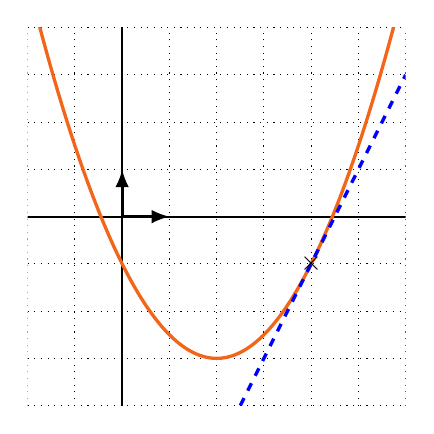
\begin{tikzpicture}[scale=0.6]
\clip (-2,-4) rectangle (6,4);
\draw [thin, dotted] (-2,-4) grid (6,4);
\draw [thick] (-4,0)--(7,0);
\draw [thick] (0,-4) -- (0,5);
\draw [very thick,->,>=latex] (0,0)--(0,1);
\draw [very thick,->,>=latex] (0,0)--(1,0);
\draw [very thick, ocre,domain=-3:6,samples=100] plot (\x,{\x*\x/2-2*\x-1});
\draw [very thick, blue, dashed,domain=-3:6] plot (\x,2*\x-9);
\draw [thick] (4,-1) node {$\times$};
\end{tikzpicture}
\end{center}
\end{minipage}
 \end{example}



\subsection{Variations d'une fonction}

\begin{proposition}Soit $f$ une fonction dérivable sur un intervalle $I$.
\begin{itemize}
\item Si, pour tout $x\in I$, $f'(x) \geqslant 0$, alors $f$ est croissante sur $I$.
\item Si, pour tout $x\in I$, $f'(x) \leqslant 0$, alors $f$ est décroissante sur $I$.
\item Si, pour tout $x\in I$, $f'(x) =0$, alors $f$ est constante sur $I$.
\end{itemize}\end{proposition}

\begin{example}On considère la fonction $f:x\mapsto (x^2-3x+1)\exp(3x+1)$ étudiée précédemment. On a vu que pour tout réel $x$, on a $f'(x)=(3x^2-7x)\exp(3x+1)=x(3x-7)\exp(3x+1)$.

$f'(x)$ étant écrite sous forme factorisée, on peut alors construire le tableau de signes de $f'$ et en déduire les variations de $f$.

\begin{center}
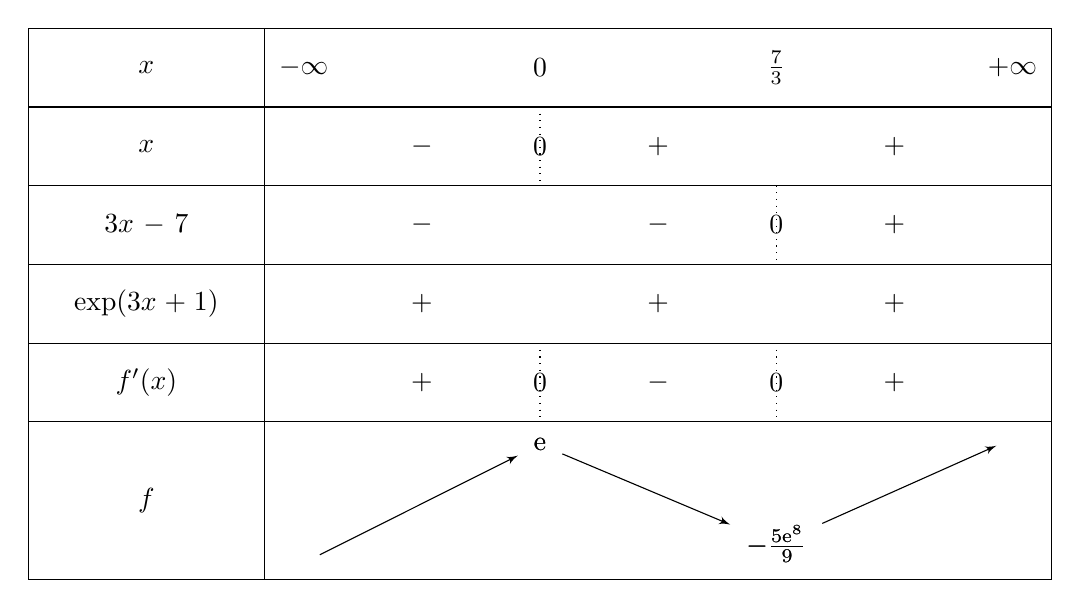
\begin{tikzpicture}[scale=1]
\tikzset{node style/.style = {inner sep = 2pt, outer sep = 2pt}}
   \tkzTabInit[lgt=3]{$x$ / 1 , $x$/1, $3x-7$/1, $\exp(3x+1)$/1, $f'(x)$/1, $f$ / 2}{$-\infty$, $0$, $\frac{7}{3}$,$+\infty$}
   \tkzTabLine{,-,z, +, , +, }
   \tkzTabLine{,-,, -, z, +, }
   \tkzTabLine{,+,, +, , +, }
   \tkzTabLine{,+,z, -, z, +, }
   \tkzTabVar{-/$ $,+/$\e$,-/$-\frac{5\e^8}{9}$,+/$ $}
\end{tikzpicture}\end{center}

\end{example}
\vspace{-0.5cm}


\section{Dérivée seconde}

\begin{definition}[Dérivée seconde] Soit $f$ une fonction dérivable sur un intervalle $I$ telle que sa fonction dérivée $f'$ est également dérivable sur $I$ (on dit également  que $f$ est deux fois dérivable sur $I$).

On appelle fonction \textit{dérivée seconde} de $f$ la fonction dérivée de $f'$. Cette fonction est notée $f''$.
\[ \text{Pour tout } x \in I, \, f''(x)=(f')'(x).\]\end{definition}

\begin{example}Pour tout réel $x$, on pose $f(x)=(2x+1)\e^{3x-2}$. Posons, pour tout réel $x$, $u_1(x)=2x+1$ et $v_1(x)=\e^{3x-2}$.
\begin{itemize}
\item $u_1$ est dérivable sur $\mathbb{R}$ et pour tout réel $x$, $u_1'(x)=2$.
\item $v_1$ est dérivable sur $\mathbb{R}$ et pour tout réel $x$, $v_1'(x)=3\e^{3x-2}$.
\end{itemize}
Ainsi, $f$ est dérivable sur $\mathbb{R}$ et pour tout réel $x$,
\[ f'(x)=u_1'(x) \times v_1(x) + u_1(x) \times v_1'(x) =  2 \times \e^{3x-2} + (2x+1) \times 3\e^{3x-2}=(6x+5)\e^{3x-2}.\]
Posons alors, pour tout réel $x$, $u_2(x)=6x+5$ et $v_2(x)=e^{3x-2}$.
\begin{itemize}
\item $u_2$ est dérivable sur $\mathbb{R}$ et pour tout réel $x$, $u_2'(x)=6$.
\item $v_2$ est dérivable sur $\mathbb{R}$ et pour tout réel $x$, $v_2'(x)=3e^{3x-2}$.
\end{itemize}
Ainsi, $f'$ est dérivable sur $\mathbb{R}$ et pour tout réel $x$,
\[ f''(x)=u_2'(x) \times v_2(x) + u_2(x) \times v_2'(x) =  6 \times e^{3x-2} + (6x+5) \times 3e^{3x-2}=(24x+21)e^{3x-2}.\]
\end{example}



\section{Composition de fonctions}


\begin{definition}[Fonction composée]  Soit $I$ et $J$ deux parties de $\mathbb{R}$.\\ Soit $f$ une fonction définie sur $J$ et $g$ une fonction définie sur $I$ telle que pour tout réel $x$, $g(x) \in J$.

On définit la \textit{fonction composée} de $f$ et $g$ notée $f \circ g$ par 
\[ \text{Pour tout } x \in I, \; f \circ g (x)= f(g(x)).\]\end{definition}
 L'idée derrière la composition de fonctions est simplement d'appliquer successivement plusieurs fonctions.
 \[f \circ g \,:\, x \overset{g}{\longmapsto} g(x) \overset{f}{\longmapsto} f[g(x)]\]

\begin{example} Pour tout réel $x$, on note $f(x)=x^2$ et $g(x)=x+3$. Alors, pour tout réel $x$,
\begin{itemize}
\item $f \circ g (x)= f(g(x))=(g(x))^2=(x+3)^2$.
\item $g \circ f(x)=g(f(x)) = f(x)+3=x^2+3$.
\end{itemize}\end{example}

Attention ! En général, on n'a pas $f \circ g = g \circ f$ ! Ces deux fonctions ne sont d'ailleurs pas forcément définies sur le même ensemble.

\begin{proposition}Soit $I$ et $J$ deux intervalles, $f$ une fonction définie et dérivable sur $J$ et $g$ une fonction définie et dérivable sur $I$ telle que pour tout $x \in I$, $g(x) \in J$. Alors $f \circ g$ est dérivable et pour tout réel $x$ dans $I$,
\[ (f \circ g)' (x)= g'(x) \times (f' \circ g)(x).\]
\vspace{-0.5cm}\end{proposition}



\begin{example}On considère la fonction $f$ définie pour tout réel $x$ par $f(x)=\e^{x^2+3x-2}$. 
Pour tout réel $x$, on pose alors $u(x)=\e^x$ et $v(x)=x^2+3x-2$. Pour tout réel $x$, on a alors  $f(x)= u(v(x)) = u \circ v (x)$.

\begin{itemize}
\item $v$ est dérivable sur $\mathbb{R}$ et pour tout réel $x$, $v'(x)=2x+3$
\item $u$ est dérivable sur $\mathbb{R}$ et pour tout réel $x$, $u'(x)=\e^x$
\end{itemize}
Ainsi, $f$ est dérivable sur $\mathbb{R}$ et pour tout réel $x$, 
\[ f'(x)= v'(x) \times u'(v(x)) = (2x+3)e^{x^2+3x-2}.\]\end{example}
\begin{proposition}[Cas particuliers] Soit $u$ une fonction définie et dérivable sur un intervalle $I$
\begin{itemize}
\item Pour tout entier naturel $n$, $u^n$ est dérivable sur $I$ et $(u^n)'=nu'u^{n-1}$.
\item $e^u$ est dérivable sur $I$ et $(\e^u)'=u' \times \e^u$.
\item Si pour tout réel $x\in I$, $u(x)>0$, alors $\sqrt{u}$ est dérivable sur $I$ et $(\sqrt{u})' = \dfrac{u'}{2\sqrt{u}}$.
\item Si pour tout réel $x$, $u(x) \neq 0$, $\dfrac{1}{u}$ est dérivable sur $I$ et $\left(\dfrac{1}{u}\right)=-\dfrac{u'}{u^2}$.
\end{itemize}\end{proposition}

\begin{example}Pour tout réel $x$, posons $f(x)=(4x+1)^9$.

Pour tout réel $x$, on pose $u(x)=4x+1$. $u$ est dérivable sur $\mathbb{R}$. Or, $f=u^9$.

 Ainsi, $f$ est dérivable sur $\mathbb{R}$ et $f'=9\times u' \times u^8$, c'est-à-dire que pour tout réel $x$, on a
\[ f'(x)= 9 \times 4 \times (4x+1)^{9-1}=36 \times (4x+1)^8.\]\end{example}

\begin{example}Pour tout réel $x$, posons $f(x)=\dfrac{1}{x^2+1}$. 

Pour tout réel $x$, on pose alors $u(x)=x^2+1$. $u$ est dérivable sur $\mathbb{R}$ et ne s'annule pas. Or, $f=\dfrac{1}{u}$.

 Ainsi, $f$ est dérivable sur $\mathbb{R}$ et $f'=-\dfrac{u'}{u^2}$, c'est-à-dire que pour tout $x\in \mathbb{R}$, on a
\[ f'(x)=- \dfrac{2x}{(x^2+1)^2}.\]\end{example}

\begin{example}On considère la fonction $f$ définie pour tout réel $x\in[-2;2]$ par $f(x)=\sqrt{4-x^2}$.

Bien que la fonction $f$ soit définie sur l'intervalle fermé $[-2;2]$, elle n'est en revanche dérivable que sur l'intervalle ouvert $]-2;2[$. Pour tout réel $x\in]-2;2[$, on a
\[f'(x)=\dfrac{-2x}{2\sqrt{4-x^2}}=-\dfrac{x}{\sqrt{4-x^2}}.\]\end{example}

\chapter{Exercices}
\setcounter{section}{0}
\section*{Rappels sur la dérivation}

\begin{exercise}[topic=der01]Dériver les fonctions suivantes, en précisant leur domaine de définition et de dérivation.

\renewcommand{\arraystretch}{2}
\begin{tabularx}{\linewidth}{XX}
 $f_1 : x \mapsto 5x^3+2x^2-3x+1$ &
$f_2 : x \mapsto 8x^7+\dfrac{4}{x^2}$ \\
 $f_3 : x \mapsto 2x^4 + \e^{3x-1}$ &
 $f_4 : x \mapsto (5x^2+2x-1)\e^x$ \\
$f_5 : x \mapsto (1-6x^2)\e^{3x+2}$ &
$f_6 : x \mapsto \dfrac{\e^x}{x}$ \\
$f_7 : x \mapsto \dfrac{x^2+3x+1}{x-5}$ &
$f_8 : x \mapsto \dfrac{x+\e^3}{\e^x}$
\end{tabularx}\end{exercise}

\begin{solution} \textbf{a.}  Pour tout réel $x$, $f_1'(x)=5\times 3x^2 + 2 \times 2x -3 = 15x^2+4x-3$.

\textbf{b.} Pour tout réel non nul $x$, $f_2'(x)=8\times 7x^6 + 4 \times \left(-\dfrac{2}{x^3}\right)=56x^6-\dfrac{8}{x^3}$.\\
Remarque : en mettant au même dénominateur, on a $f'_2(x)=\dfrac{56x^9-8}{x^3}$.

\textbf{c.} Pour tout réel $x$, $f_3'(x)=2\times 4x^3+3e^{3x-1}=8x^3+3\e^{3x-1}$.

\textbf{d.} Pour tout réel $x$, on pose $u(x)=5x^2+2x-1$ et $v(x)=\e^x$.
\begin{itemize}
\item $u$ est dérivable sur $\mathbb{R}$ et pour tout réel $x$, $u'(x)=10x+2$.
\item $v$ est dérivable sur $\mathbb{R}$ et pour tout réel $x$, $v'(x)=\e^x$.
\end{itemize}
Ainsi, puisque $f_4=uv$, $f$ est dérivable sur $\mathbb{R}$ et $f_4'=u'v+uv'$. Pour tout réel $x$, on a donc
\[ f_4'(x)=(10x+2)\e^x+(5x^2+2x-1)\e^x=(5x^2+12x+1)\e^x.\]

\textbf{e.} Pour tout réel $x$, on pose $u(x)=1-6x^2$ et $v(x)=\e^{3x+2}$.
\begin{itemize}
\item $u$ est dérivable sur $\mathbb{R}$ et pour tout réel $x$, $u'(x)=-12x$.
\item $v$ est dérivable sur $\mathbb{R}$ et pour tout réel $x$, $v'(x)=3\e^{3x+2}x$.
\end{itemize}
Ainsi, puisque $f_5=uv$, $f_5$ est dérivable sur $\mathbb{R}$ et $f'=u'v+uv'$. Pour tout réel $x$, on a donc
\[ f_5'(x)=-12x\e^{3x+2}+(1-6x^2)\times 3\e^{3x+2}=[-12x+(1-6x^2)\times 3] \e^{3x+2}=(-18x^2-12x+3)\e^{3x+2}.\]

\textbf{f.} Pour tout réel non nul $x$, on pose $u(x)=\e^x$ et $v(x)=x$.
\begin{itemize}
\item $u$ est dérivable sur $]-\infty;0[$ et $]0;+\infty[$, et pour tout réel non nul $x$, $u'(x)=\e^x$.
\item $v$ est dérivable et ne s'annule pas sur $]-\infty;0[$ et $]0;+\infty[$, et pour tout réel non nul $x$, $v'(x)=1$.
\end{itemize}
Ainsi, puisque $f_6=\dfrac{u}{v}$, $f$ est dérivable sur $]-\infty;0[$ et $]0;+\infty[$ et $f_6'=\dfrac{u'v-uv'}{v^2}$. Pour tout réel non nul $x$, on a donc
\[ f_6'(x)=\dfrac{\e^x\times x-\e^x\times 1}{x^2}=\dfrac{(x-1)\e^x}{x^2}.\]

\textbf{g.} Pour tout réel $x\neq 5$, on pose $u(x)=x^2+3x+1$ et $v(x)=x-5$.
\begin{itemize}
\item $u$ est dérivable sur $]-\infty;5[$ et $]5;+\infty[$, et pour tout réel $x\neq 5$, $u'(x)=2x+3$.
\item $v$ est dérivable et ne s'annule pas sur $]-\infty;5[$ et $]5;+\infty[$, et pour tout réel $x\neq 5$, $v'(x)=1$.
\end{itemize}
Ainsi, puisque $f=\dfrac{u}{v}$, $f$ est dérivable sur $]-\infty;5[$ et $]5;+\infty[$ et $f'=\dfrac{u'v-uv'}{v^2}$. Pour tout réel $x\neq 5$, on a donc
\[ f_7'(x)=\dfrac{(2x+3)(x-5)-(x^2+3x+1)}{(x-5)^2}=\dfrac{2x^2-10x+3x-15-x^2-3x-1}{(x-5)^2}=\dfrac{x^2-10x-16}{(x-5)^2}.\]
\newpage
\textbf{h.} Pour tout réel $x$, on pose $u(x)=x+\e^3$ et $v(x)=\e^x$.
\begin{itemize}
\item $u$ est dérivable sur $\mathbb{R}$, et pour tout réel $x$, $u'(x)=1$.
\item $v$ est dérivable et ne s'annule pas sur $\mathbb{R}$, et pour tout réel $x$, $v'(x)=\e^x$.
\end{itemize}
Ainsi, puisque $f=\dfrac{u}{v}$, $f$ est dérivable sur $\mathbb{R}$ et $f'=\dfrac{u'v-uv'}{v^2}$. Pour tout réel $x$, on a donc
\[ f_8'(x)=\dfrac{1\times e^x -(x+e^3)e^x}{(e^x)^2}=\dfrac{(-x+1-e^3)e^x}{(e^x)^2}=\dfrac{-x+1-e^3}{e^x}.\]\end{solution}



\begin{exercise}[topic=der01] On considère la fonction $f:x\mapsto x^3+3x^2-45x+21$.
\begin{enumerate}
\item $f$ est dérivable pour tout $x\in\mathbb{R}$. Que vaut $f'(x)$ ?
\item Construire le tableau de signes de $f'$ et en déduire le tableau de variations de $f$.
\end{enumerate}\end{exercise}

\begin{solution}Pour tout réel $x$, on a $f'(x)=3x^2+6x-45$.

Notons $\Delta$ le discriminant du polynôme $3x^2+6x-45$. On a $\Delta = 6^2-4\times 3 \times (-45)=576>0$.

Le polynôme $3x^2+6x-45$ admet donc deux racines réelles distinctes
\[ x_1 = \dfrac{-6-\sqrt{576}}{2\times 3}=-5 \quad \text{et}\quad x_2= \dfrac{-6+\sqrt{576}}{2\times 3}=3.\]
Par ailleurs, le signe d'un polynôme est celui de son coefficient dominant (ici, 3) à l'extérieur des racines. Il est du signe opposé entre les racines. On peut alors dresser le tableau de signe de $f'$ et en déduire le tableau de variations de $f$.

\begin{center}
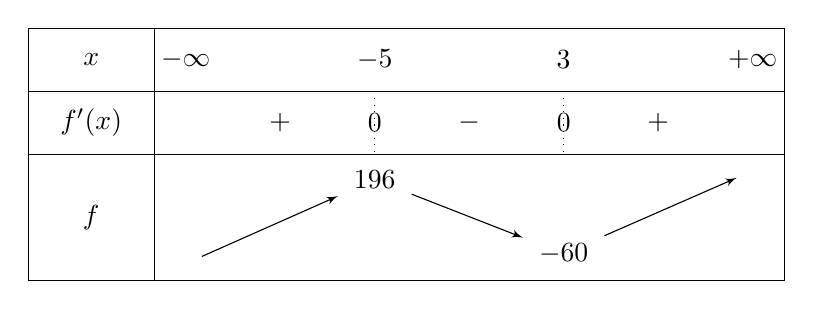
\begin{tikzpicture}[scale=0.8]
   \tkzTabInit{$x$ / 1 ,$f'(x)$/1,$f$/2}{$-\infty$, $-5$, $3$, $+\infty$}
      \tkzTabLine{, +, z, -,z,+,  }
   \tkzTabVar{-/$ $,+/$196$,-/$-60$,+/$ $}
\end{tikzpicture}
\end{center}\end{solution}

\begin{exercise}[topic=der01]On considère la fonction $f$ définie pour tout réel $x$ par $f(x)=\dfrac{10x+4}{5x^2+1}$
\begin{enumerate}
\item Justifier que $f$ est dérivable sur $\mathbb{R}$. Exprimer $f'(x)$ pour tout réel $x$.
\item Construire le tableau de variations de $f$ sur $\mathbb{R}$
\end{enumerate}\end{exercise}

\begin{solution}Pour tout réel $x$, on pose $u(x)=10x+4$ et $v(x)=5x^2+1$
\begin{itemize}
\item $u$ est dérivable sur $\mathbb{R}$, et pour tout réel $x$, $u'(x)=10$
\item $v$ est dérivable et ne s'annule pas sur $\mathbb{R}$, et pour tout réel $x$, $v'(x)=10x$
\end{itemize}
Ainsi, puisque $f=\dfrac{u}{v}$, $f$ est dérivable sur $\mathbb{R}$ et $f'=\dfrac{u'v-uv'}{v^2}$. Pour tout réel $x$, on a donc
\[ f'(x)=\dfrac{10\times(5x^2+1)-(10x+4)\times 10x}{(5x^2+1)^2}=\dfrac{-50x^2-40x+10}{(5x^2+1)^2}\]

Pour tout réel $x$, $(5x^2+1)^2>0$. Il ne reste qu'à étudier le signe de $-50x^2-40x+10$. C'est un polynôme du second degré dont le discriminant vaut $(-40)^2-4\times 10 \times (-50)=3600>0$. Ce polynôme admet donc deux racines réelles distinctes qui sont
\[ x_1=\dfrac{-(-40)+\sqrt{3600}}{2\times (-50)}=-1 \quad \text{et}\quad x_2=\dfrac{-(-40)-\sqrt{3600}}{2\times (-50)}=\dfrac{1}{5}=0.2\] 
On peut alors construire le tableau de signes de $f'$ et en déduire le tableau de variations de $f$. 


\begin{center}
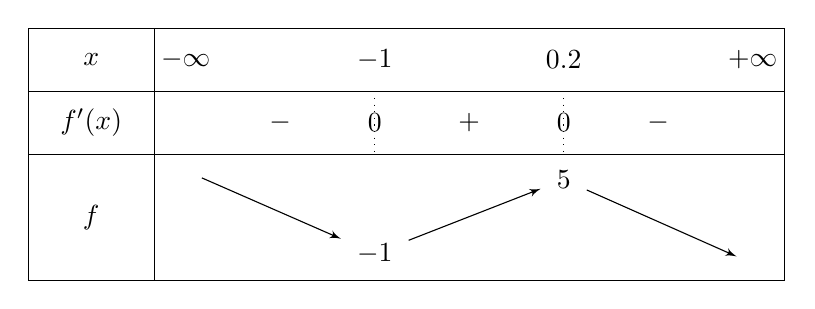
\begin{tikzpicture}[scale=0.8]
   \tkzTabInit{$x$ / 1,$f'(x)$/1,$f$/2}{$-\infty$, $-1$, $0.2$, $+\infty$}
      \tkzTabLine{, -,z, +,z,-,  }
   \tkzTabVar{+/$ $,-/$-1$,+/$5$,-/$ $}
\end{tikzpicture}
\end{center}
\end{solution}


\begin{exercise}[topic=der01]Pour tout réel $x \neq -1$, on pose $f(x)=\dfrac{\e^x}{1+x}$.
\begin{enumerate}
\item Justifier que $f$ est dérivable sur $]-\infty ; -1[$ et sur $]-1;+\infty[$ et que pour tout réel $x$ dans ces intervalles
\[f'(x)=\dfrac{x\,\e^x}{(1+x)^2}.\]
\item Étudier le signe de $f'(x)$ et en déduire le tableau de variations de $f$.
\end{enumerate}\end{exercise}

\begin{solution}Pour tout réel $x\neq -1$, on pose $u(x)=\e^x$ et $v(x)=1+x$.
\begin{itemize}
\item $u$ est dérivable sur $]-\infty;-1[$ et $]-1;+\infty[$, et pour tout réel $x\neq -1$, $u'(x)=\e^x$.
\item $v$ est dérivable et ne s'annule pas sur $]-\infty;-1[$ et $]-1;+\infty[$, et pour tout réel $x\neq -1$, $v'(x)=1$.
\end{itemize}
Ainsi, puisque $f=\dfrac{u}{v}$, $f$ est dérivable sur $]-\infty;-1[$ et $]-1;+\infty[$ et $f'=\dfrac{u'v-uv'}{v^2}$. Pour tout réel $x\neq -1$,
\[ f'(x)=\dfrac{\e^x \times (1+x)-\e^x\times 1}{(1+x)^2}=\dfrac{x\e^x}{(1+x)^2}\]

Pour tout réel $x\neq -1$, $(1+x)^2> 0$ et $\e^x >0$. $f'(x)$ est donc du signe de $x$ (hormis en $-1$, valeur interdite).

\begin{center}
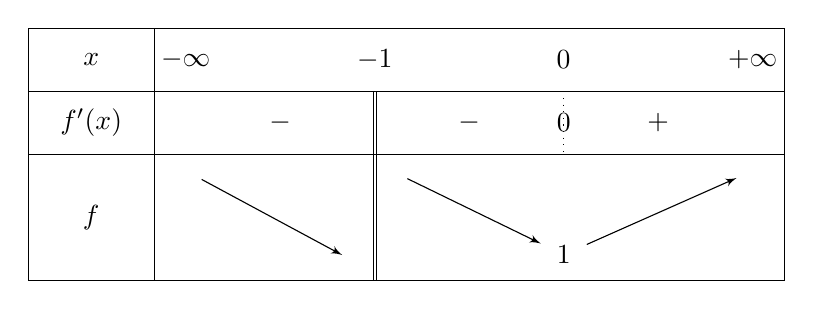
\begin{tikzpicture}[scale=0.8]
   \tkzTabInit{$x$ / 1,$f'(x)$/1,$f$/2}{$-\infty$, $-1$, $0$, $+\infty$}
      \tkzTabLine{, -,d, -,z,+,  }
   \tkzTabVar{+/$ $,-D+/$ $,-/$1$,+/$ $}
\end{tikzpicture}
\end{center}\end{solution}




\begin{exercise}[topic=der01, subtitle={}]Construire le tableau de variations de la fonction $f:x\mapsto (-x^2+x+1)\e^{1-3x}$ définie sur $\mathbb{R}$.\end{exercise}

\begin{solution}Pour tout réel $x$, on pose $u(x)=-x^2+x+1$ et $v(x)=\e^x$.
\begin{itemize}
\item $u$ est dérivable sur $\mathbb{R}$ et pour tout réel $x$, $u'(x)=-2x+1$
\item $v$ est dérivable sur $\mathbb{R}$ et pour tout réel $x$, $v'(x)=\e^x$
\end{itemize}
Ainsi, puisque $f=uv$, $f$ est dérivable sur $\mathbb{R}$ et $f'=u'v+uv'$. Pour tout réel $x$, on a donc
\[ f'(x)=(-2x+1)\e^x+(-x^2+x+1)\e^x=(-x^2-x+2)\e^x.\]
Pour tout réel $x$, $\e^x>0$. Il ne reste donc qu'à étudier le signe de $-x^2-x+2$. Il s'agit d'un polynôme du second degré. Son discriminant vaut $\Delta = (-1)^2-4\times(-1)\times 2 = 9>0$. Le polynôme $-x^2-x+2$ admet donc deux racines réelles distinctes
\[ x_1=\dfrac{-(-1)-\sqrt{9}}{2\times(-1)}=1 \quad\text{et}\quad x_2=\dfrac{-(-1)+\sqrt{9}}{2\times(-1)}=-2.\]
On peut alors construire le tableau de signes de $f'$ et en déduire le tableau de variations de $f$. 


\begin{center}
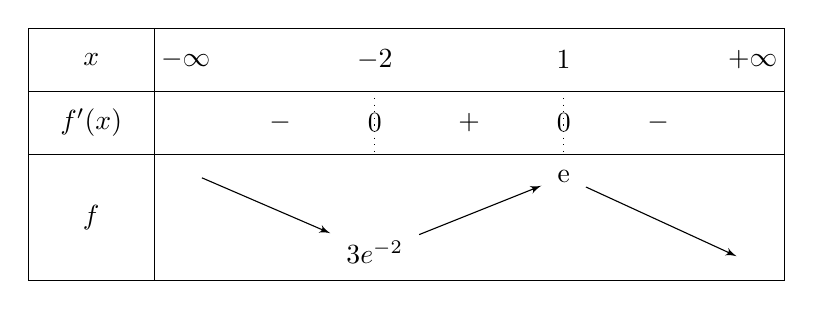
\begin{tikzpicture}[scale=0.8]
   \tkzTabInit{$x$ / 1,$f'(x)$/1,$f$/2}{$-\infty$, $-2$, $1$, $+\infty$}
      \tkzTabLine{, -,z, +,z,-,  }
   \tkzTabVar{+/$ $,-/$3e^{-2}$,+/$\e$,-/$ $}
\end{tikzpicture}
\end{center}

\end{solution}




\begin{exercise}[topic=der01, subtitle={(Centres étrangers 2024)}]On considère la suite \((u_n)\) définie par \(u_0=0,1\) et, pour tout entier naturel \(n\), $u_{n+1}=2u_n\e^{-u_n}$
\begin{enumerate}
 	\item Déterminer le sens de variations de la fonction \(f\) définie pour tout réel \(x\in [0;1] \) par \(f(x)=2x\e^{-x}\).
 	\item Montrer par récurrence que pour tout entier naturel \(n\), on a $0 \leqslant u_n \leqslant u_{n+1} \leqslant 1$.
\end{enumerate}
\end{exercise}

\begin{solution}
 La fonction \(f\) est dérivable comme produit de fonctions dérivables sur \([0;1]\)
 
 De plus, pour tout réel \(x\in[0;1]\), on a
\[f'(x) = 2 \times \e^{-x}+2x\times(-\e^{-x})=(2-2x)\e^{-x}.\]
Or, pour tout \(x\in [0;1]\), $\e^{-x}>0$. Par ailleurs, si $0\leqslant x \leqslant 1$, on a $0 \geqslant -2x \geqslant -2$ et donc $2 \geqslant 2-2x \geqslant 0$. En particulier, pour tout $x\in [0;1]$, $2-2x\geqslant 0$.

Ainsi, pour tout réel positif $x\in [0;1]$, \(f'(x) \geqslant 0\). \(f\) est donc croissante sur \([0;1]\).

Pour tout entier naturel \(n\), on considère la proposition \(\mathcal{P}(n)\) : « \(0 \leqslant u_n \leqslant u_{n+1} \leqslant 1\) ».
\begin{itemize}
\item \textbf{Initialisation :} Pour \(n=0\), on a \(u_0=0,1\) et \(u_1 = 2 \times 0,1 \times \e^{-0,1}\simeq 0,18\). On a bien \(0 \leqslant u_0 \leqslant u_1 \leqslant 1\). \(\mathcal{P}(0)\) est vraie.
\item \textbf{Hérédité} : Soit \(n\in\mathbb{N}\). Supposons que \(\mathcal{P}(n)\) est vraie, c'est-à-dire \(0 \leqslant u_n \leqslant u_{n+1} \leqslant 1\).La fonction \(f\) étant croissante sur \([0;1] \), on peut l'appliquer à cette inégalité sans en changer le sens. Ainsi,
\[f(0) \leqslant f(u_n) \leqslant f(u_{n+1}) \leqslant f(1).\]Or, \(f(0)=0\), \(f(u_n)=u_{n+1}\), \(f(u_{n+1})=u_{n+2}\) et \(f(1)=\dfrac{2}{e}\leqslant 1\). Il en vient que
\[0 \leqslant u_{n+1} \leqslant u_{n+2} \leqslant \dfrac{2}{e} \leqslant 1.\]
\(\mathcal{P}(n+1)\) est donc vraie.
\item \textbf{Conclusion} : \(\mathcal{P}(0)\) est vraie. \(\mathcal{P}\) est héréditaire. Par récurrence, \(\mathcal{P}(n)\) est vraie pour tout entier \(n\in\mathbb{N}\).\end{itemize}
\end{solution}








\begin{exercise}[topic=der01] A l'aide d'une étude de fonction, montrer que pour tout réel $x$, on a $\e^x \geqslant 1+x$ \end{exercise}

\begin{solution}Pour tout réel $x$, on pose $f(x)=\e^x-x-1$. $f$ est dérivable sur $\mathbb{R}$ et pour tout réel $x$, $f'(x)=\e^x-1$. On sait par ailleurs que $e^x \geqslant 1 \Leftrightarrow x\geqslant 0$. On en déduit le tableau de signes de $f'$ et le tableau de variations de $f$.

\begin{center}
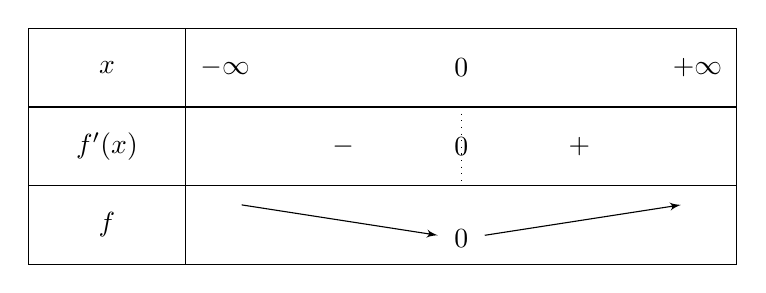
\begin{tikzpicture}[scale=1]
   \tkzTabInit{$x$ / 1,$f'(x)$/1,$f$/1}{$-\infty$, $0$, $+\infty$}
      \tkzTabLine{, -,z, +,  }
   \tkzTabVar{+/$ $,-/$0$,+/$ $}
\end{tikzpicture}
\end{center}

On a en effet $f(0)=\e^0-0-1=0$. Ainsi, pour tout réel $x$, $f(x)\geqslant 0$, soit $\e^x-x-1 \geqslant 0$ ou $\e^x \geqslant 1+x$.

Graphiquement, cela signifie que la courbe de la fonction exponentielle est toujours au-dessus de sa tangente en 0.\end{solution}

\printcollection{der01}

\section*{Dérivée seconde}


\begin{exercise}[topic=der02]Pour chacune des fonctions suivantes, deux fois dérivables sur l'intervalle mentionné, donner une expression de la dérivée seconde.

\begin{tabularx}{\linewidth}{XX}
 $f_1 : x \mapsto 6x^2+2x-1$ sur $\mathbb{R}$ &
 $f_2 : x \mapsto 3x^2+2x-\dfrac{3}{x}$, sur $]-\infty;0[$  \\
 $f_3 : x \mapsto x^2e^{3x+1}$,  sur $\mathbb{R}$ &
 $f_4 : x \mapsto \dfrac{3x^2-1}{x}$, sur $]-\infty;0[$ \\
 $f_5 : x \mapsto (1-6x^2)e^{3x+2}$, sur $\mathbb{R}$ &
 $f_6 : x \mapsto \dfrac{e^x}{x}$, sur $]0;+\infty[$
\end{tabularx}\end{exercise}

\begin{solution}Pour tout réel $x$, $f_1'(x)=12x+2$ et $f_1''(x)=12$.

Pour tout réel $x<0$, $f_2'(x)=6x+\dfrac{3}{x^2}$ et $f_2''(x)=6-\dfrac{6}{x^3}$.

Pour tout réel $x$, on pose $u_1(x)=x^2$ et $v_1(x)=\e^{3x+1}$. $u_1$ et $v_1$ sont dérivables sur $\mathbb{R}$. $f$ est donc également dérivable sur $\mathbb{R}$ et $f'=u_1'v_1+u_1v_1'$. Ainsi, pour tout réel $x$,
\[ f_3'(x)= 2x \times \e^{3x+1} + x^2 \times 3\e^{3x+1} = (3x^2+2x)\e^{3x+1}.\]

Pour tout réel $x$, on pose $u_2(x)=3x^2+2x$ et $v_2(x)=\e^{3x+1}$. $u_2$ et $v_2$ sont dérivables sur $\mathbb{R}$, $f_3'$ l'est donc également et $f_3''=u_2'v_2+u_2v_2'$. Ainsi, pour tout réel $x$,
\[f_3''(x)=(6x+2)\e^{3x+1}+(3x^2+2x)\times 3\e^{3x+1}=(3x^2+12x+2)\e^{3x+1}.\]

On peut remarquer que pour tout réel $x<0$, $f_4(x)=\dfrac{3x^2}{x}-\dfrac{1}{x}=3x-\dfrac{1}{x}$. \\Ainsi, pour tout réel $x<0$, $f_4'(x)=3+\dfrac{1}{x^2}$ et $f_4''(x)=-\dfrac{2}{x^3}$.

Pour tout réel $x$, on pose $u_1(x)=1-6x^2$ et $v_1(x)=\e^{3x+2}$.
\begin{itemize}
\item $u_1$ est dérivable sur $\mathbb{R}$ et pour tout réel $x$, $u_1'(x)=-12x$.
\item $v_1$ est dérivable sur $\mathbb{R}$ et pour tout réel $x$, $v_1'(x)=3\e^{3x+2}x$.
\end{itemize}
Ainsi, puisque $f_5=u_1v_1$, $f_5$ est dérivable sur $\mathbb{R}$ et $f_5'=u_1'v_1+u_1v_1'$. Pour tout réel $x$, on a donc
\[ f_5'(x)=-12x\e^{3x+2}+(1-6x^2)\times 3\e^{3x+2}=[-12x+(1-6x^2)\times 3] \e^{3x+2}=(-18x^2-12x+3)\e^{3x+2}.\]

Pour tout réel $x$, on pose alors $u_2(x)=-18x^2-12x+3$ et $v_2(x)=\e^{3x+2}$. $u_2$ et $v_2$ sont dérivables sur $\mathbb{R}$, $f_5'$ l'est donc également. Pour tout réel $x$,
\[ f_5''(x)= (-36x-12)\e^{3x+2} + (-18x^2-12x+3) \times 3\e^{3x+2}=(-54x^2-72x-3)\e^{3x+2}.\]

Pour tout réel $x>0$, on pose $u_1(x)=\e^x$ et $v_1(x)=x$. $u_1$ et $v_1$ sont dérivables sur $]0;+\infty[$ et $v$ ne s'annule pas sur cet intervalle. Ainsi, $f_6$ est dérivable sur $]0;+\infty[$ et pour tout réel $x$,
\[ f_6'(x)= \dfrac{e^x \times x - e^x \times 1}{x^2}=\dfrac{(x-1)e^x}{x^2}.\]

Posons alors, pour tout réel $x>0$, $u_2(x)=(x-1)\e^x$ et $v_2(x)=x^2$. $v_2$ est dérivable et ne s'annule pas sur $]0;+\infty[$. Par ailleurs, $u_1$ est dérivable sur $]0;+\infty[$ car c'est un produit de fonctions dérivables sur cet intervalle. Pour tout réel $x>0$
\[ u_1'(x)= 1 \times \e^x + (x-1)\e^x =x\e^x\]

Ainsi, pour tout réel $x>0$
\[ f_6''(x)=\dfrac{x\e^x \times x^2-(x-1)\e^x \times 2x}{x^4}=\dfrac{(x^3-2x^2+2x)\e^x}{x^4}=\dfrac{(x^2-2x+2)\e^x}{x^3}\]
\newpage
\end{solution}




\begin{exercise}[topic=der02] On considère la fonction $f$ définie pour tout $x\in\mathbb{R}$ par $f(x)=3x^4+16x^3-66x^2-360x+120$.
\begin{enumerate}
\item Soit $x$ un réel. Que vaut $f'(x)$ ?
\item On note $f''$ la dérivée de $f'$. Que vaut $f''(x)$ ?
\item Construire la tableau de signes de $f''$.
\item En déduire le tableau de variations de $f'$.
\item On indique de plus que $f'(-5)=f'(3)=f'(-2)=0$. Construire le tableau de signes de $f'$ et en déduire le tableau de variations de $f$.
\end{enumerate}
\end{exercise}

\begin{solution}
 Pour tout réel $x$, $f'(x)=12x^3+48x^2-132x-360$ et $f''(x)=36x^2+96x-132$.
 
$f''$ est une fonction polynôme du second degré dont le discriminant vaut $96^2-4 \times 36 \times (-132)=28224>0$. L'équation $f''(x)=0$ admet donc deux solutions réelles
\[x_1=\dfrac{-96-\sqrt{28224}}{2 \times 36}=-\dfrac{11}{3} \quad \text{et}x_2=\dfrac{-96+\sqrt{28224}}{2 \times 36}=1.\]

On peut alors construire le tableau de signes de $f''$. Par ailleurs, $f''$ étant la dérivée de $f'$, on en déduit le tableau de variations de $f'$.

\begin{center}
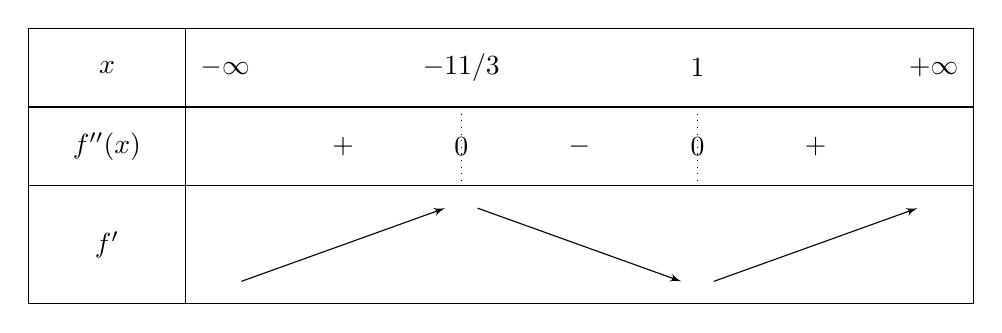
\begin{tikzpicture}[scale=1]
   \tkzTabInit{$x$ / 1,$f''(x)$/1,$f'$/1.5}{$-\infty$, $-11/3$, $1$, $+\infty$}
      \tkzTabLine{,+,z, -,z, +,  }
   \tkzTabVar{-/$ $,+/$ $,-/$ $,+/$ $}
\end{tikzpicture}
\end{center}

Puisque $f'$ est croissante sur $]-\infty;5]$ et que $f'(5)=0$, on en déduit que pour tout réel $x\leqslant 5$, $f'(x)\leqslant 0$. En raisonnant de même sur les autres intervalles, on en déduit le tableau de signes de $f'$ et donc le tableau de variations de $f$.

\begin{center}
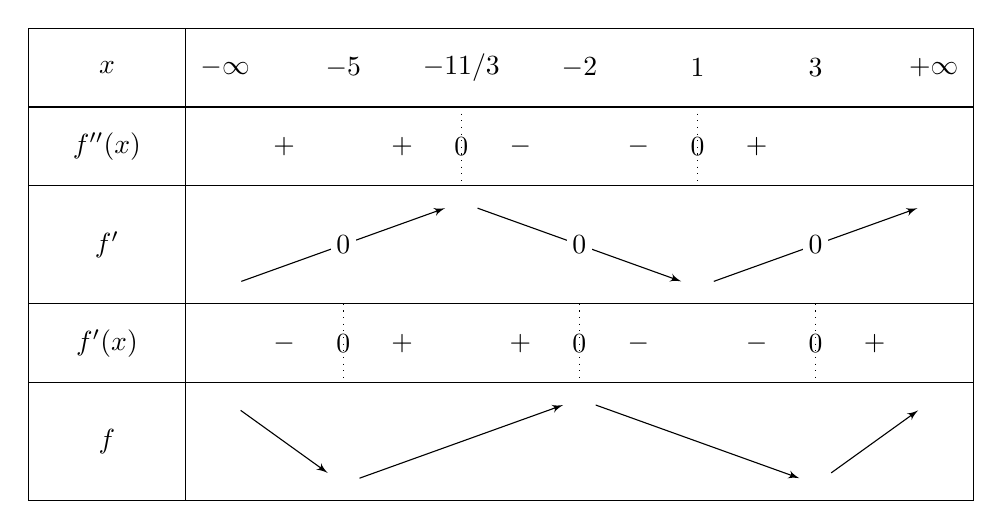
\begin{tikzpicture}[scale=1]
   \tkzTabInit[espcl=1.5]{$x$ / 1,$f''(x)$/1,$f'$/1.5,$f'(x)$/1,$f$/1.5}{$-\infty$, $-5$, $-11/3$, $-2$, $1$, $3$, $+\infty$}
      \tkzTabLine{,+,,+,z, -,,-,z, +,  }
   \tkzTabVar{-/$ $,R,+/$ $,R,-/$ $,R,+/$ $}
   \tkzTabIma{1}{3}{2}{$0$}
   \tkzTabIma{3}{5}{4}{$0$}
   \tkzTabIma{5}{7}{6}{$0$}
   \tkzTabLine{,-,z,+,,+,z,-,,-,z,+,}
   \tkzTabVar{+/$ $,-/$ $,R,+/$ $,R,-/$ $,+/$ $}
\end{tikzpicture}
\end{center}\end{solution}





\begin{exercise}[topic=der02]On considère une fonction $f$ deux fois dérivable. On a représenté ci-dessous la courbe de $f'$ dans un repère orthonormé.

\begin{center}
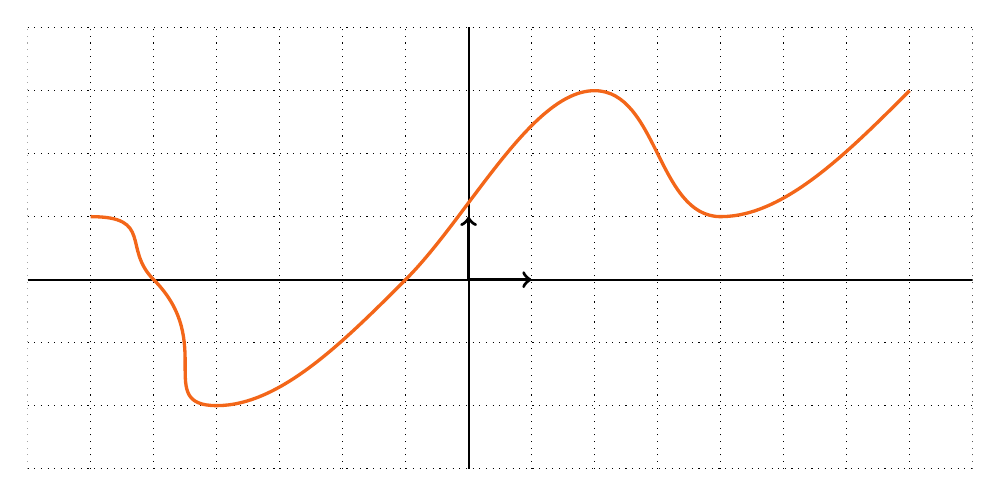
\begin{tikzpicture}[scale=0.8]
\clip (-7,-3) rectangle (8,4);
\draw [ thin, dotted] (-7,-3) grid (9,5);
\draw [thick] (-7,0)--(9,0);
\draw [thick] (0,-3)--(0,5);
\draw [->, very thick] (0,0)--(1,0);
\draw [->,very thick] (0,0)--(0,1);

\draw [ocre, very thick] (-6,1) .. controls (-5,1) and (-5.5,0.5) .. (-5,0)
.. controls (-4,-1) and (-5,-2) .. (-4,-2) .. controls (-3,-2) and (-2,-1) ..
(-1,0) .. controls (0,1) and (1,3) .. (2,3) .. controls (3,3) and (3,1) ..
(4,1) .. controls (5,1) and (6,2) .. (7,3);

\end{tikzpicture}
\end{center}

On sait par ailleurs que $f(-6)=-1$, $f(-5,5)=0$ et $f(-1)=2$. Construire le tableau de signes de $f''$ et $f$ sur l'intervalle $[-6;7]$.

\end{exercise}

\begin{solution}\(f^{\prime\prime}\) est la dérivée de \(f'\). Les variations de \(f'\) nous donnent donc le signe de \(f^{\prime\prime}\).
\begin{center}
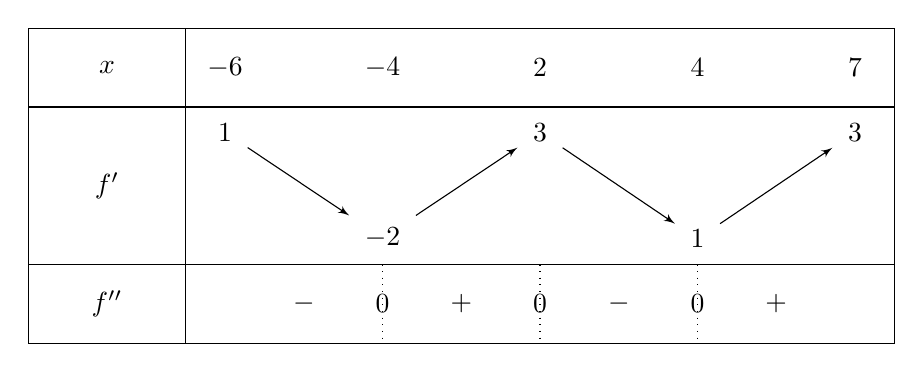
\begin{tikzpicture}[scale=1]
\tkzTabInit[espcl=2]{$x$ / 1 , $f'$ / 2, $f^{\prime\prime}$ / 1}{$-6$, $-4$, $2$,$4$, $7$}
\tkzTabVar{+/$1$,-/$-2$,+/$3$,-/$1$,+/$3$}
\tkzTabLine{,-,z,+,z, -, z, +, }
\end{tikzpicture}
\end{center}

Par ailleurs, à l'aide du signe de \(f'\), on peut construire le tableau de variations de \(f\). Les informations sur les valeurs extrêmes de \(f\) nous permettent de construire son tableau de signes.
\begin{center}
\begin{tikzpicture}[scale=1]
\tkzTabInit[espcl=2]{$x$ / 1 , $f'(x)$ / 1, $f$ / 2, $f(x)$/1}{$-6$, $-5.5$, $-5$,$-1$, $7$}
\tkzTabLine{,+,,+,z,-,z, -, z, +, }
\tkzTabVar{-/$ $,R,+/$\geqslant 0$,-/$2$,+/$ $}
\tkzTabIma{1}{3}{2}{$0$}
\tkzTabLine{,-,z,+,,+,, +, , +, }
\end{tikzpicture}
\end{center}
\end{solution}




\begin{exercise}[topic=der02]Soit $f$ et $g$ deux fonctions deux fois dérivables sur un intervalle $I$. Justifier que $(fg)$ est deux fois dérivable sur $I$ et exprimer $(fg)''$ en fonction de $f$, $g$ et de leurs dérivées.\end{exercise}

\begin{solution}Si $f$ et $g$ sont dérivables, alors $fg$ l'est également et $(fg)'=f'g+fg'$. Si de plus $f'$ et $g'$ sont dérivables, alors $f'g$ et $fg'$ le sont également et
\begin{itemize}
\item $(f'g)'=f''g+f'g'$ ;
\item $(fg')'=f'g'+fg''$.
\end{itemize}
Ainsi, $(fg)'$ est dérivable et $(fg)''=f''g+f'g'+f'g'+fg''=f''g+2f'g'+fg''$.\end{solution}



\begin{exercise}[topic=der02]Soit $a$ et $b$ deux réels. Pour tout réel $x$, on pose $f(x)=(ax+b)\e^x$.
\begin{enumerate}
\item Justifier que $f$ est deux fois dérivable sur $\mathbb{R}$ puis donner une expression de $f'(x)$ et $f''(x)$.
\item Montrer que pour tout réel $x$, $f''(x)-2f'(x)+f(x)=0$.
\end{enumerate}\end{exercise}

\begin{solution}Les fonctions $x\mapsto ax+b$ et $x\mapsto \e^x$ sont deux fois dérivables sur $\mathbb{R}$. Leur produit est donc deux fois dérivable sur $\mathbb{R}$. 

Pour tout réel $x$, $f'(x)=a\e^x+(ax+b)\e^x=(ax+a+b)e^x$ et $f''(x)=a\e^x+(ax+a+b)\e^x=(ax+2a+b)\e^x$. Ainsi, pour tout réel $x$,
\[f''(x)-2f'(x)+f(x)=(ax+2a+b)\e^x-2(ax+a+b)\e^x+(ax+b)\e^x\]
et donc
\[f''(x)-2f'(x)+f(x)=(ax+2a+b-2ax-2a-2b+ax+b)\e^x=0\]\end{solution}



\begin{exercise}[topic=der02]Soit $f$ une fonction définie sur un intervalle $I$ et $n$ un entier naturel. Lorsqu'il est possible de dériver $n$ fois la fonction $f$ sur $I$, on dit que $f$ est $n$ fois dérivable et on note $f^{(n)}$ la fonction obtenue en dérivant $n$ fois. On a alors $f^{(0)}=f$,  $f^{(1)}=f'$, $f^{(2)}=f''$...
\begin{enumerate}
\item On considère la fonction $f:x\mapsto x \e^x$. Montrer par récurrence que, pour tout entier naturel $n$, $f$ est $n$ fois dérivable et pour tout réel $x$, $f^{(n)}(x)=(x+n)\e^x$. 
\item On considère la fonction $g:x\mapsto x \e^{-x}$. Montrer par récurrence que, pour tout entier naturel $n$, $g$ est $n$ fois dérivable et pour tout réel $x$, $g^{(n)}(x)=(-1)^n(x-n)\e^x$ .
\end{enumerate}\end{exercise}

\begin{solution}Pour tout entier naturel \(n\), on considère la proposition \(P(n)\) : « \(f\) est \(n\) fois dérivable sur \(\mathbb{R}\) et pour tout réel \(x\), \(f^{(n)}(x)=(x+n)\e^x\) ».
\begin{itemize}
\item \textbf{Initialisation} : \(f\) est bien dérivable 0 fois et pour tout réel \(x\), \(f^{(0)}(x)=f(x)=(x+0)\e^x\).
\item\textbf{ Hérédité} : Soit \(n\) un entier naturel. Supposons que \(P(n)\) est vraie. Alors \(f\) est \(n\) fois dérivable sur \(\mathbb{R}\) et pour tout réel \(x\), \(f^{(n)}(x)=(x+n)\e^x\). \(f^{(n)}\) est dérivable sur \(\mathbb{R}\) car c'est le produit de deux fonctions dérivables sur \(\mathbb{R}\). \(f\) est donc \(n+1\) fois dérivable sur \(\mathbb{R}\). Par ailleurs, pour tout réel \(x\),
\[f^{(n+1)}(x) = (f^{(n)})'(x)=\e^x+(x+n)\e^x=(x+n+1)\e^x.\]
\(P(n+1)\) est donc vraie.
\item \textbf{Conclusion} : \(P(0)\) est vraie, \(P\) est héréditaire. Par récurrence, \(P(n)\) est vraie pour tout entier naturel \(n\).
\end{itemize}

Pour tout entier naturel \(n\), on considère la proposition \(P(n)\) : « \(g\) est \(n\) fois dérivable sur \(\mathbb{R}\) et pour tout réel \(x\), \(g^{(n)}(x)=(-1)^n (x-n)\e^{-x}\) ».
\begin{itemize}
\item \textbf{Initialisation} : \(g\) est bien dérivable 0 fois et pour tout réel \(x\), \(g^{(0)}(x)=g(x)=(-1)^0(x-0)\e^{-x}\). \(P(0)\) est vraie.
\item \textbf{Hérédité} : Soit \(n\) un entier naturel. Supposons que \(P(n)\) est vraie. Alors \(g\) est \(n\) fois dérivable sur \(\mathbb{R}\) et pour tout réel \(x\), \(g^{(n)}(x)=(-1)^n(x-n)\e^{-x}\). \(g^{(n)}\) est dérivable sur \(\mathbb{R}\) car c'est le produit de deux fonctions dérivables sur \(\mathbb{R}\). \(g\) est donc \(n+1\) fois dérivable sur \(\mathbb{R}\). Par ailleurs, pour tout réel \(x\),
\begin{eqnarray*}g^{(n+1)}(x) = (g^{(n)})'(x)&=&(-1)^n \times(\e^{-x}+(x-n)\times(-\e^{-x}))\\& =& (-1)^n (1-x+n) \e^{-x} \\&=&(-1)^n \times (-(x-n-1))\e^{-x}\\&=&(-1)^{n+1}(x-(n+1))\e^{-x.}\end{eqnarray*} 
\(P(n+1)\) est donc vraie.
\item \textbf{Conclusion} : \(P(0)\) est vraie, \(P\) est héréditaire. Par récurrence, \(P(n)\) est vraie pour tout entier naturel \(n\).
\end{itemize}
\end{solution}

\printcollection{der02}

\section*{Composition de fonctions}

\begin{exercise}[topic=der03]Pour tout réel $x$, on pose $f(x)=x^2+1$, $g(x)=3x+2$ et $h(x)=2-x$.\\
\noindent Donner une expression de $(f \circ g) (x)$, $(g \circ f) (x)$, $(h \circ g) (x)$ et   $(f \circ g \circ h) (x)$.
\end{exercise}

\begin{solution}Pour tout réel $x$,
\begin{itemize}
\item  $(f \circ g) (x)=f(g(x))=g(x)^2+1=(3x+2)^2+1=9x^2+12x+5$.
\vskip5pt
\item   $(g \circ f) (x)=3f(x)+2=3(x^2+1)+2=3x^2+5$ .
\vskip5pt
\item  $(h \circ g) (x)=2-g(x)=2-(3x+2)=-3x$.
\vskip5pt
\item $(f \circ g \circ h) (x)=(f \circ g)(h(x))=(3h(x)+2)^2+1=(8-3x)^2+1=9x^2-48x+65$.
\end{itemize}
\end{solution}

\begin{exercise}[topic=der03]Exprimer chacune des fonctions suivantes comme la composition de deux fonctions « usuelles ». On ne se souciera pas des domaines de définition.

\renewcommand{\arraystretch}{2}
\begin{tabularx}{\linewidth}{XXX}
 $f_1 : x \mapsto \e^{1+x^2}$&
 $f_2 : x \mapsto (3x+8)^7$&
  $f_3 : x \mapsto \sqrt{1+\e^x}$ \\
\end{tabularx}
\end{exercise}

\begin{solution}
Pour tout réel $x$, on pose $u(x)=\e^x$ et $v(x)=1+x^2$. On a alors $f_1=u \circ v$.

Pour tout réel $x$, on pose $u(x)=x^7$ et $v(x)=3x+8$. On a alors $f_2=u \circ v$.

Pour tout réel positif $x$ positif, on pose $u(x)=\sqrt(x)$. Pour tout réel $x$, on pose $v(x)=1+\e^x$. On a alors $f_3=u \circ v$.
\end{solution}

\begin{exercise}[topic=der03]Soit $f$ une fonction définie sur un ensemble $E$. On dit que $f$ est une involution de $E$ si pour tout $x\in E$, $(f \circ f)(x)=x$.
\begin{enumerate}
\item Montrer que la fonction $x\mapsto \dfrac{1}{x}$ est une involution de $\mathbb{R}^*$.
\item Soit $a$ un réel. Montrer que la fonction $x\mapsto a-x$ est une involution de $\mathbb{R}$.
\item Soit $a$ et $b$ deux réels, avec $b\neq 0$. Montrer que la fonction $x\mapsto \dfrac{b}{x-a}+a$ est une involution de $\mathbb{R}\setminus \{a\}$.
\end{enumerate}\end{exercise}

\begin{solution}
Pour tout réel $x\neq 0$, $f(f(x))=\dfrac{1}{\frac{1}{x}}=x$. $f$ est bien une involution de $\mathbb{R}^*$.

Pour tout réel $x$, $f(f(x))=a-(a-x)=x$. $f$ est une involution de $\mathbb{R}$.

Pour tout réel $x\neq a$,
\[f(f(x))=\dfrac{b}{\left(\frac{b}{x-a}+a\right)-a}+a=\dfrac{b}{\dfrac{b}{x-a}}+a=x-a+a=x.\]
$f$ est une involution de $\mathbb{R}\setminus \{a\}$.\end{solution}




\begin{exercise}[topic=der03]Dériver les fonctions suivantes, dérivables sur l'intervalle donné.

\renewcommand{\arraystretch}{2}
\begin{tabularx}{\linewidth}{XX}
 $f_1 : x \mapsto (3x+2)^2$, sur $\mathbb{R}$ &
 $f_2 : x \mapsto (6x^2+3x+4)^3$,  sur $\mathbb{R}$ \\
  $f_3 : x \mapsto \e^{\sqrt{x}}$,  sur $]0;+\infty[$ &
$f_4 : x \mapsto \sqrt{2x^2-5x+7}$,sur $\mathbb{R}$ \\
  $f_5 : x \mapsto \dfrac{1}{(3x+6)^2}$, sur $]-2;+\infty[$ &
$f_6 : x \mapsto \e^{x+\frac{1}{x}}$,  sur $]-\infty;0[$ 
\end{tabularx}\end{exercise}

\begin{solution}\textbf{a.} Pour tout réel $x$, $f'_1(x)=3\times 2 (3x+2)=18x+12$.
\vskip5pt
\textbf{b.} Pour tout réel $x$, $f'_2(x)=(12x+3)\times 3(6x^2+3x+4)^2=(36x+9)(6x^2+3x+4)^2$.
\vskip5pt
\textbf{c.} Pour tout réel $x>0$, $f'_3(x)=\dfrac{1}{2\sqrt{x}}\times \e^{\sqrt{x}}$.
\vskip5pt
\textbf{d.} Pour tout réel $x$, $f'_4(x)=\dfrac{4x-5}{2\sqrt{2x^2-5x+7}}$.
\vskip5pt
\textbf{e.} Pour tout réel $x>2$, $f_5'(x)=3 \times \left(-\dfrac{2}{(3x+6)^3}\right)=-\dfrac{6}{(3x+6)^3}$.
\vskip5pt
\textbf{f.} Pour tout réel $x\neq 0$, $f'_6(x)=\left(1-\dfrac{1}{x^2}\right)\e^{x+\frac{1}{x}}$.\end{solution}




\begin{exercise}[topic=der03]On considère la fonction $f:x\mapsto \e^{3x^2+2x-1}$, définie sur $\mathbb{R}$.
\begin{enumerate}
\item Justifier que $f$ est dérivable sur $\mathbb{R}$ et calculer $f'(x)$ pour tout réel $x$.
\item Construire le tableau de variations de $f$.
\item Déterminer l'équation de la tangente à la courbe de $f$ au point d'abscisse $-1$.
\end{enumerate}
\newpage \end{exercise}

\begin{solution}Pour tout réel $x$, $f(x)=\e^{u(x)}$ avec $u(x)=3x^2+2x-1$. $u$ est dérivable sur $\mathbb{R}$, $f$ l'est donc aussi et $f'=u'e^u$. Ainsi, pour tout réel $x$, 
\[f'(x)=(6x+2)\e^{3x^2+2x-1}.\]

Pour tout réel $x$, $\e^{3x^2+2x-1}>0$, $f'(x)$ est donc du signe de $6x+2$.

\begin{center}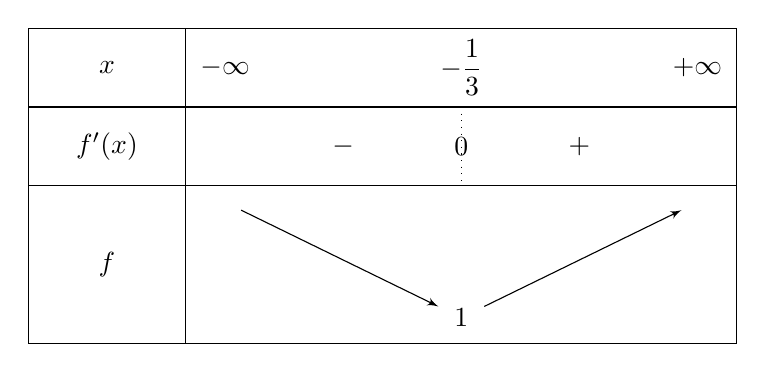
\begin{tikzpicture}[scale=1]
   \tkzTabInit{$x$ / 1 , $f'(x)$ / 1, $f$ / 2}{$-\infty$, $-\dfrac{1}{3}$, $+\infty$}
   \tkzTabLine{, -, z, +,  }
   \tkzTabVar{+/$ $,-/$1$,+/$ $}
\end{tikzpicture}
\end{center}

La tangente à la courbe de $f$ à l'abscisse $-1$ a pour équation $y=f'(-1)(x+1)+f(-1)$ soit $y=-4(x+1)+1$ ou encore $y=-4x-3$.\end{solution}




\begin{exercise}[topic=der03]Construire le tableau de variations de la fonction $f:x\mapsto \sqrt{x^2-4x+5}$, définie et dérivable sur $\mathbb{R}$  puis tracer l'allure de sa courbe représentative dans un repère orthogonal.\end{exercise}

\begin{solution}
Pour tout réel $x$, $x^2-4x+5>0$. En effet, il s'agit d'un polynôme du second degré dont le discriminant est strictement négatif. De plus, $f(x)=\sqrt{u(x)}$. Ainsi, $f$ est définie et dérivable sur $\mathbb{R}$ et $f'=\dfrac{u'}{2\sqrt{u}}$. 

Pour tout $x\in\mathbb{R}$, on a donc $f'(x)=\dfrac{2x-4}{2\sqrt{x^2-4x+5}}$. Puisque pour tout $x\in\mathbb{R}$, $\sqrt{x^2-4x+5}>0$, $f'(x)$ est du signe de $2x-4$.

\begin{minipage}{0.45\linewidth}

\begin{center}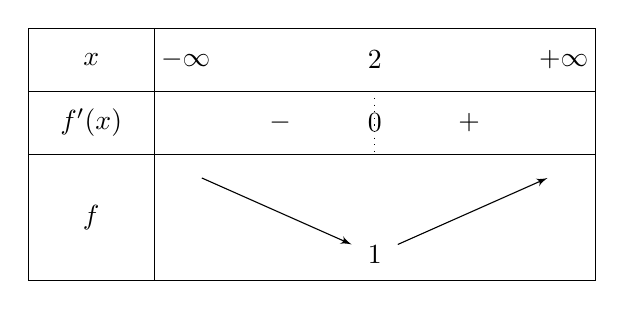
\begin{tikzpicture}[scale=0.8]
   \tkzTabInit{$x$ / 1 , $f'(x)$ / 1, $f$ / 2}{$-\infty$, $2$, $+\infty$}
   \tkzTabLine{, -, z, +,  }
   \tkzTabVar{+/$ $,-/$1$,+/$ $}
\end{tikzpicture}\end{center}

\end{minipage}\hfill\begin{minipage}{0.45\linewidth}

\begin{center}
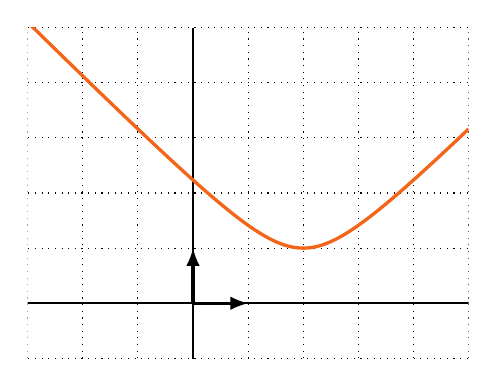
\begin{tikzpicture}[scale=0.7]
\clip (-3,-1) rectangle (5,5);
\draw [thin, dotted] (-6,-1) grid (6,5);
\draw [thick] (-4,0)--(7,0);
\draw [thick] (0,-4) -- (0,5);
\draw [very thick,->,>=latex] (0,0)--(0,1);
\draw [very thick,->,>=latex] (0,0)--(1,0);
\draw [very thick, ocre,domain=-3:5,samples=100] plot (\x,{sqrt(\x*\x-4*\x+5});
\end{tikzpicture}
\end{center}
\end{minipage}
\newpage
\end{solution}




\begin{exercise}[topic=der03]On considère la fonction $f:x\mapsto \sqrt{1-x^2}$. On note $D$ le domaine de définition de $f$ et $D'$ son domaine de dérivabilité.

\begin{enumerate}
\item Déterminer $D$ et $D'$.
\item Donner une expression de $f'(x)$ pour tout $x\in D'$.
\item Pour tout réel $x\in D$, on pose $g(x)=\e^{\sqrt{1-x^2}}$.
\begin{enumerate}
\item Justifier que $g$ est dérivable sur $D'$ et calculer $g'(x)$ pour tout $x$ dans $D'$.
\item En déduire le sens de variations de $g$ puis tracer l'allure de la courbe représentative de $g$ dans un repère orthonormé.
\end{enumerate}
\end{enumerate}\end{exercise}

\begin{solution}
\begin{enumerate}
\item  $\sqrt{1-x^2}$ existe si et seulement si $1-x^2 \geqslant 0$, c'est-à-dire $x^2 \leqslant 1$ et donc $x\in [-1;1]$. Par ailleurs, la fonction racine carrée n'est pas dérivable en zéro. Ainsi, $f$ n'est pas dérivable en $-1$ et $1$, qui sont les solutions de l'équation $1-x^2=0$. On a donc $D'=]-1;1[$.
\item Pour tout $x\in D'$, $f'(x)=\dfrac{-2x}{2\sqrt{1-x^2}}=-\dfrac{x}{\sqrt{1-x^2}}$.
\item 
\begin{enumerate}
\item On a $g=\e^f$. Or, $f$ est dérivable sur $D'$, $g$ l'est donc également et pour tout réel $x$ de $D'$,
\[g'(x)=f'(x) \times \e^{f(x)}=-\dfrac{x\e^{\sqrt{1-x^2}}}{\sqrt{1-x^2}}.\]



\item Puisque pour tout réel $x\in D$, $\sqrt{1-x^2}>0$ et $e^{-\sqrt{1-x^2}}>0$, $g'(x)$ est du signe de $-x$.

\begin{center}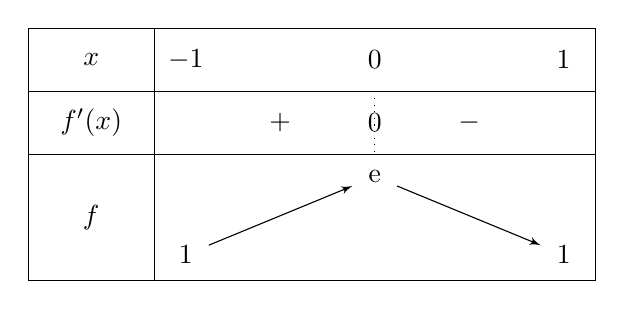
\begin{tikzpicture}[scale=0.8]
   \tkzTabInit{$x$ / 1 , $f'(x)$ / 1, $f$ / 2}{$-1$, $0$, $1$}
   \tkzTabLine{, +, z, -,  }
   \tkzTabVar{-/$1$,+/$\e$,-/$1$}
\end{tikzpicture}
\end{center}


\item On trace l'allure de la courbe représentative de $g$ dans un repère orthonormé.

\begin{center}
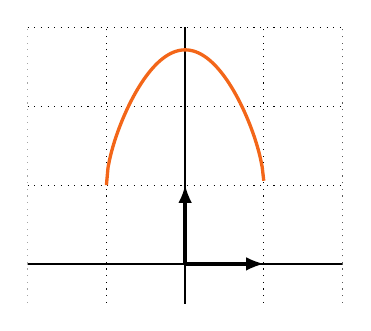
\begin{tikzpicture}[scale=1]
\clip (-2,-0.5) rectangle (2,3);
\draw [thin, dotted] (-2,-1) grid (2,3);
\draw [thick] (-4,0)--(7,0);
\draw [thick] (0,-4) -- (0,5);
\draw [very thick,->,>=latex] (0,0)--(0,1);
\draw [very thick,->,>=latex] (0,0)--(1,0);
\draw [very thick, ocre,domain=-1:1,samples=100] plot (\x,{exp(sqrt(1-\x*\x)});
\end{tikzpicture}
\end{center}

\end{enumerate}
\end{enumerate}
\end{solution}




\begin{exercise}[topic=der03]On considère la fonction $f:x\mapsto \e^{x^2+2x-5}$, définie et deux fois dérivable sur $\mathbb{R}$. 
\begin{enumerate}
\item Construire le tableau de variation de $f$.
\item  Déterminer une expression de $f''(x)$ pour tout réel $x$.
\end{enumerate}
\end{exercise}


\begin{solution}$f$ est dérivable sur $\mathbb{R}$ et pour tout réel $x$, $f'(x)=(2x+2)\e^{x^2+2x-5}$ qui est du signe de $2x+2$.

\begin{center}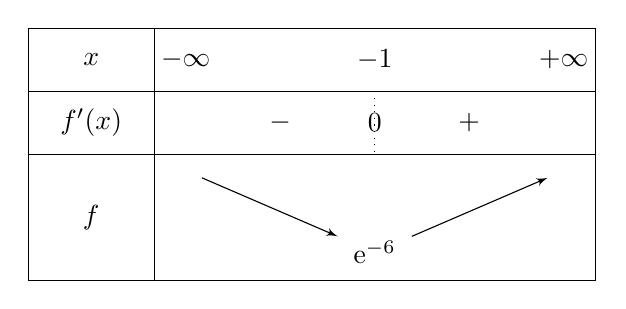
\begin{tikzpicture}[scale=0.8]
   \tkzTabInit{$x$ / 1 , $f'(x)$ / 1, $f$ / 2}{$-\infty$, $-1$, $+\infty$}
   \tkzTabLine{, -, z, +,  }
   \tkzTabVar{+/$ $,-/$\e^{-6}$,+/$ $}
\end{tikzpicture}
\end{center}

En utilisant la dérivée d'un produit, pour tout réel $x$, on a
\[f''(x)=2 \times \e^{x^2+2x-5} + (2x+2) \times (2x+2)\e^{x^2+2x-5} = (4x^2+8x+6)\e^{x^2+2x-5}.\]\end{solution}




\begin{exercise}[topic=der03]Pour tout réel $x$, on pose $f(x)=\left(\dfrac{x^2-2x-3}{2}\right)^2$.
\begin{enumerate}
\item Justifier que $f$ est dérivable sur $\mathbb{R}$ et calculer $f'(x)$ pour tout réel $x$.
\item En déduire les variations de $f$ sur $\mathbb{R}$ et tracer la courbe représentative de $f$ dans un repère orthonormé.
\item Justifier que $f$ est deux fois dérivable sur $\mathbb{R}$. Donner une expression de $f''(x)$ pour tout réel $x$.
\end{enumerate}\end{exercise}

\begin{solution}Pour tout réel $x$, on pose $u(x)=\dfrac{x^2-2x-3}{2}$. $u$ est dérivable sur $\mathbb{R}$ et $f=u^2$. $f$ est donc dérivable sur $\mathbb{R}$ et $f'=2u'u$. Pour tout réel $x$,
\[f'(x)=2 \times (x-1) \times \dfrac{x^2-2x-3}{2}=(x-1)(x^2-2x-3).\] 

Le polynôme $x^2-2x-3$ s'annule en $-1$ et en $3$. Ainsi, pour tout réel $x$, $f'(x)=(x-1)(x+1)(x-3)$. On peut alors construire le tableau de signes de $f'$ et le tableau de variations de $f$.



\begin{center}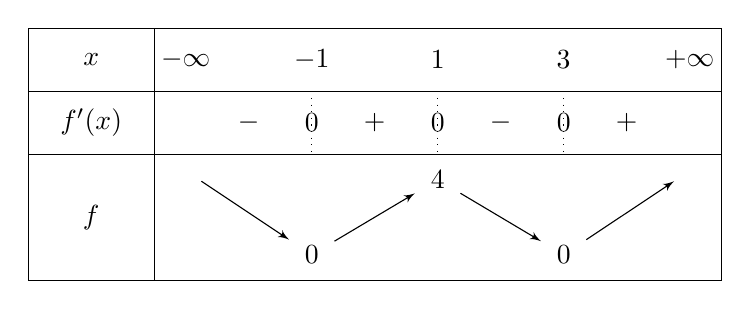
\begin{tikzpicture}[scale=0.8]
   \tkzTabInit[espcl=2]{$x$ / 1 , $f'(x)$ / 1, $f$ / 2}{$-\infty$, $-1$, $1$,$3$, $+\infty$}
   \tkzTabLine{,-,z,+,z, -, z, +,  }
   \tkzTabVar{+/$ $,-/$0$,+/$4$,-/$0$,+/$ $}
\end{tikzpicture}
\end{center}




\begin{center}
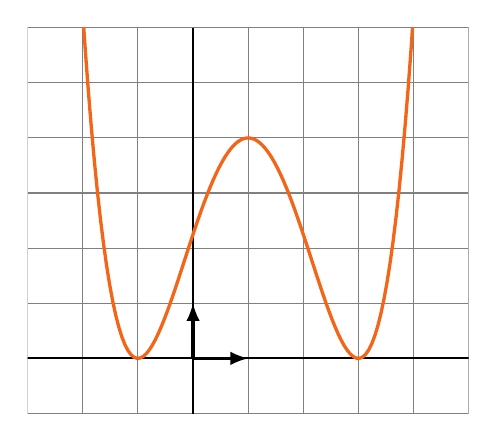
\begin{tikzpicture}[scale=0.7]
\clip (-3,-1) rectangle (5,6);
\draw [thin,gray] (-3,-4) grid (5,8);
\draw [thick] (-4,0)--(7,0);
\draw [thick] (0,-4) -- (0,6);
\draw [very thick,->,>=latex] (0,0)--(0,1);
\draw [very thick,->,>=latex] (0,0)--(1,0);
\draw [very thick, ocre,domain=-4:7,samples=200] plot (\x,{(\x*\x-2*\x-3)^2/4});
\end{tikzpicture}
\end{center}



$f'$ est le produit de deux fonctions dérivables sur $\mathbb{R}$ et est donc dérivable sur $\mathbb{R}$. Pour tout réel $x$,
\[f''(x)=1 \times (x^2-2x-3) + (x-1) \times (2x-2)=3x^2-6x-1.\]\end{solution}




\begin{exercise}[topic=der03]Donner une expression de la dérivée seconde de la fonction $f:x\mapsto \e^{1/x}$ sur $]0;+\infty[$.\end{exercise}

\begin{solution}Pour tout réel $x>0$, on pose $u(x)=\dfrac{1}{x}$. $u$ est dérivable sur $]0;+\infty[$ et $f=\e^u$. $f$ est donc dérivable sur $]0;+\infty[$ et $f'=u'\e^u$. Ainsi, pour tout réel $x>0$, $f'(x)=-\dfrac{\e^{1/x}}{x^2}$.

$f'$ est également dérivable comme quotient de fonctions dérivables dont le dénominateur ne s'annule pas sur $]0;+\infty[$. Par ailleurs, pour tout réel $x>0$,
\[f''(x)=-\left(\dfrac{-\dfrac{\e^{1/x}}{x^2}\times x^2 - \e^{1/x} \times 2x}{(x^2)^2}\right)=\dfrac{(2x+1)\e^{1/x}}{x^4}.\]\end{solution}


\begin{exercise}[topic=der03]On considère la fonction \(f:x\mapsto \dfrac{\e^x}{\sqrt{x}}\), définie sur \(]0;+\infty[\).

\begin{enumerate}
\item Justifier que \(f\) est dérivable sur \(]0;+\infty [\) et que pour tout réel \(x>0\), $f'(x)=\dfrac{(2x-1)\e^x}{2x\sqrt{x}}$.
\item Construire le tableau de variations de la fonction \(f\) sur \(]0;+\infty[\).
\end{enumerate}

On considère désormais la fonction \(g:x\mapsto \dfrac{\e^{x^2+x+1}}{\sqrt{x^2+x+1}}\). 

On peut remarquer que pour tout réel \(x\), \(g(x)=f(x^2+x+1)\).
\begin{enumerate}
\setcounter{enumi}{2}
\item Justifier que \(g\) est définie et dérivable sur \(\mathbb{R}\) et que pour tout réel \(x\),
\[g'(x)=\dfrac{(2x+1)(2x^2+2x+1)\e^{x^2+x+1}}{2(x^2+x+1)\sqrt{x^2+x+1}}.\]
\textbf{Indication }: ne pas utiliser la dérivée d'un quotient vous épargnera de longs et pénibles calculs.
\item Construire le tableau de variations de \(g\) sur \(\mathbb{R}\).\end{enumerate}\end{exercise}

\begin{solution}\vspace{0pt}
\begin{enumerate}\item  Les fonctions \(x \mapsto \e^x\) et \(x\mapsto \sqrt{x}\) sont dérivables sur \(]0;+\infty[\). De plus, la fonction \(x \mapsto \sqrt{x}\) ne s'annule pas sur cet intervalle. Ainsi, \(f\) est dérivable sur \(]0;+\infty[\) et, pour tout réel \(x>0\), on a 
\[f'(x)= \dfrac{\e^x \times \sqrt{x} - \e^x \times \frac{1}{2\sqrt{x}}}{\sqrt{x}^2} = \dfrac{1}{x} \times \dfrac{\e^x\sqrt{x} \times 2 \sqrt{x} - \e^x}{2\sqrt{x}} = \dfrac{(2x-1)\e^x}{2x\sqrt{x}}.\]

\item Pour tout réel \(x>0\), \(f'(x)\) est du signe de \((2x-1)\).

\begin{center}
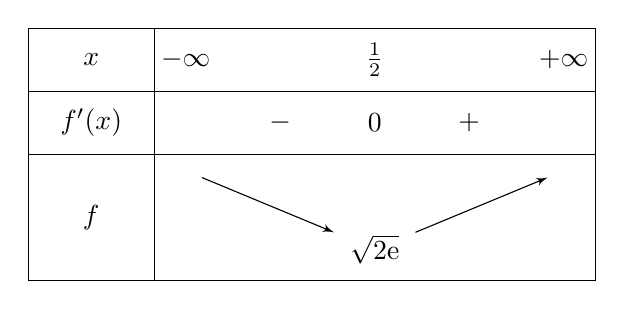
\begin{tikzpicture}[scale=0.8]
   \tkzTabInit{$x$ / 1 , $f'(x)$/1, $f$ / 2}{$-\infty$, $\frac{1}{2}$,$+\infty$}
   \tkzTabLine{,-,0,+ ,  }
   \tkzTabVar{+/$ $,-/$\sqrt{2\e}$,+/$ $}
\end{tikzpicture}
\end{center}


\item La fonction \(u : x\mapsto x^2+x+1\) est une fonction dérivable sur \(\mathbb{R}\). Par ailleurs, pour tout réel \(x\), \(x^2+x+1>0\) (on calcule le discriminant du polynôme \(x^2+x+1\), celui-ci est strictement négatif). Ainsi, \(g\) est dérivable sur \(\mathbb{R}\) et pour tout réel \(x\),

\[g'(x)= u'(x) \times f'(u(x)) = (2x+1) \times \dfrac{(2(x^2+x+1)-1)e^{x^2+x+1}}{2(x^2+x+1)\sqrt{x^2+x+1}}\]
et donc
\[g'(x)= \dfrac{(2x+1)(2x^2+2x+1)\e^{x^2+x+1}}{2(x^2+x+1)\sqrt{x^2+x+1}} .\]
\item \(g'(x)\) est du signe de \((2x+1)\) (on vérifie que pour tout réel \(x\), \(2x^2+2x+1 > 0\) à l'aide du discriminant par exemple).

\begin{center}
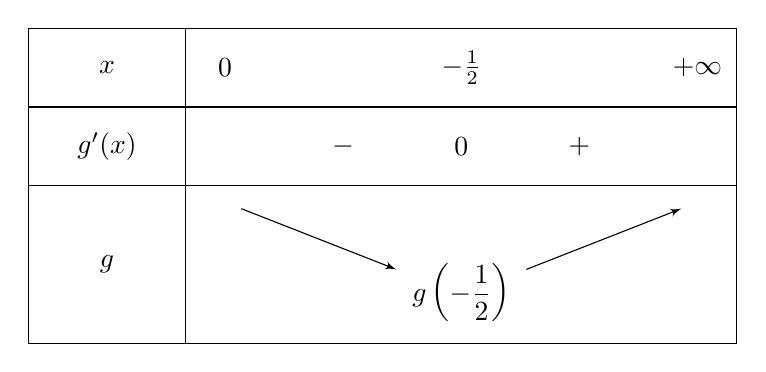
\begin{tikzpicture}[scale=1]
   \tkzTabInit{$x$ / 1 , $g'(x)$/1, $g$ / 2}{$0$, $-\frac{1}{2}$,$+\infty$}
   \tkzTabLine{,-,0,+ ,  }
   \tkzTabVar{+/$ $,-/$g\left(-\dfrac{1}{2}\right)$,+/$ $}
\end{tikzpicture}
\end{center}
\end{enumerate}
\end{solution}

\printcollection{der03}

\chapter{Correction des exercices}


\section*{Rappels sur la dérivation}
\printsolutions[collection={der01}, headings={false} ]

\section*{Dérivée seconde}

\printsolutions[collection={der02}, headings={false} ]

\section*{Composition de fonctions}

\printsolutions[collection={der03}, headings={false} ]





\end{document}